\documentclass{elsarticle}

\usepackage[utf8x]{inputenc}
\usepackage[table]{xcolor}
\usepackage{amsmath}
\usepackage{amssymb}
\usepackage{url}
\usepackage{graphicx}
\usepackage[table]{xcolor}
\usepackage{tabularx}
\usepackage{multirow,makecell}
\usepackage{float,lscape}
\usepackage[ruled,linesnumbered,vlined]{algorithm2e}
\usepackage{microtype}
\usepackage{lscape} 
\usepackage{tabularx} 
\usepackage{tabulary} 
\usepackage[binary-units=true]{siunitx}

\definecolor{redorange}{rgb}{0.878431, 0.235294, 0.192157}
\definecolor{lightblue}{rgb}{0.552941, 0.72549, 0.792157}
\definecolor{clearyellow}{rgb}{0.964706, 0.745098, 0}
\definecolor{clearorange}{rgb}{0.917647, 0.462745, 0}
\definecolor{mildgray}{rgb}{0.54902, 0.509804, 0.47451}
\definecolor{softblue}{rgb}{0.643137, 0.858824, 0.909804}
\definecolor{bluegray}{rgb}{0.141176, 0.313725, 0.603922}
\definecolor{lightgreen}{rgb}{0.709804, 0.741176, 0}
\definecolor{redpurple}{rgb}{0.835294, 0, 0.196078}
\definecolor{midblue}{rgb}{0, 0.592157, 0.662745}
\definecolor{clearpurple}{rgb}{0.67451, 0.0784314, 0.352941}
\definecolor{browngreen}{rgb}{0.333333, 0.313725, 0.145098}
\definecolor{darkestpurple}{rgb}{0.396078, 0.113725, 0.196078}
\definecolor{greypurple}{rgb}{0.294118, 0.219608, 0.298039}
\definecolor{darktruqoise}{rgb}{0, 0.239216, 0.298039}
\definecolor{darkbrown}{rgb}{0.305882, 0.211765, 0.160784}
\definecolor{midgreen}{rgb}{0.560784, 0.6, 0.243137}
\definecolor{darkred}{rgb}{0.576471, 0.152941, 0.172549}
\definecolor{darkpurple}{rgb}{0.313725, 0.027451, 0.470588}
\definecolor{darkestblue}{rgb}{0, 0.156863, 0.333333}
\definecolor{lightpurple}{rgb}{0.776471, 0.690196, 0.737255}
\definecolor{softgreen}{rgb}{0.733333, 0.772549, 0.572549}
\definecolor{offwhite}{rgb}{0.839216, 0.823529, 0.768627}

\title{SAT Competition 2020\tnoteref{title}}
\tnotetext[title]{\url{satcompetition.github.io/2020}}

\author[jku]{Nils Froleyks}
\ead{nils.froleyks@jku.at}
\author[cmu]{Marijn Heule}
\ead{marijn@cmu.edu}
\author[kit]{Markus Iser}
\ead{markus.iser@kit.edu}
\author[uh]{Matti J\"arvisalo}
\ead{matti.jarvisalo@helsinki.fi}
\author[ctu]{Martin Suda} 
\ead{martin.suda@cvut.cz}

\address[jku] {
Institute for Formal Models and Verification, Johannes Kepler University, Austria\\
{\tt nils.froleyks@jku.at}\\[1em]
}


\address[cmu] {
Computer Science Department, Carnegie Mellon University, USA\\
{\tt marijn@cmu.edu}\\[1em]
}

\address[kit] {
Department of Informatics, Karlsruhe Institute of Technology, Germany \\
{\tt markus.iser@kit.edu}\\[1em]
}

\address[uh] {
HIIT, Department of Computer Science, University of Helsinki, Finland
{\tt matti.jarvisalo@helsinki.fi}\\[1em]
}

\address[ctu] {
Czech Technical University in Prague, Czech Republic\\
{\tt martin.suda@cvut.cz}\\[1em]
}


\newcommand{\todo}[1]{{\color{purple}Todo: #1}}
\newcommand{\solver}[1]{\texttt{#1}}
\newcommand{\solbert}[1]{\underline{\solver{#1}}}
\newcommand{\solverine}[1]{\texttt{\textls*[-70]{#1}}}

% Stack a variable number of arguments:
\makeatletter
\newcommand{\stack}[1]{%
\begin{tabular}{@{}l@{}}#1\checknextarg}
\newcommand{\checknextarg}{\@ifnextchar\bgroup{\gobblenextarg}{\end{tabular}}}
\newcommand{\gobblenextarg}[1]{\\#1\@ifnextchar\bgroup{\gobblenextarg}{\end{tabular}}}
\makeatother

\begin{document}

\begin{abstract}
The SAT Competitions constitute a well-established series of yearly open international algorithm implementation competitions
focusing on the Boolean satisfiability (or propositional satisfiability, SAT) problem. 
In this article, we provide
a detailed account on the 2020 instantiation of the SAT Competition, including the 
 new competition tracks and benchmark selection procedures, overview of solving strategies implemented in top-performing solvers, 
and a more detailed analysis of the empirical data obtained from running the competition.
%SAT Competition 2020 stands in the tradition of the series of annual competitive events which motivate and assess the progress in SAT solving. 
%This competition was special as it introduced the new cloud track where SAT Solvers that run on hundreds of processors could compete. 
%Another novelty was the application-specific sub-track of the main track, 
%where solvers competed in solving benchmark instances from one specific domain only, and in this year that was the planning domain. 
%We used new tools to select and distribute benchmark instances and their attributes. 
%In this paper we provide a description of the well-known and the new competition tracks and how we organized them. 
%It follows then a detailed analysis of the results and the strategies of the award winning solvers. 
\end{abstract}

\begin{keyword}
SAT, Boolean satisfiability, SAT Competition, SAT solvers, empirical evaluation,
benchmarking
\end{keyword}

\maketitle

\section{Introduction}

From what was once mainly the archetypal intractable (in particular NP-complete) problem, propositional satisfiability 
(or Boolean satisfiability, SAT) has flourished in practice into a success story of modern computer science.
This is due to advances in SAT solvers, i.e., implementations of decision procedures for SAT, which form today a 
central computational tool for solving real-world problem instances of various kinds of NP-hard search and optimization problems.
With standardized input formats, readily-available APIs for incremental applications,
and certified proof logging and checking capabilities, applications of SAT solver technology
have branched from first breakthrough applications in automated planning, test pattern generation and hardware verification
to thousands of different application settings. 

The success of SAT would not be without the persistent efforts of the SAT community to further develop the performance and robustness
of SAT solvers. The SAT Competition series, which a history dating back to early 90s, aims to support and provide further incentives 
for maintaining and furthering this progress. Organized yearly as an international open event, the SAT competitions (and their variants
in the form of SAT Races and SAT Challenge) have a consistent track record of receiving tens of solver submissions yearly, submitted
by the community at large for obtaining a snapshot of the current state-of-the-art in practical SAT solving. Alongside participating solvers,
the competition invite through open calls submissions of benchmark instances representing in particular new interesting applications 
scenarios of SAT solvers. Indeed, in addition to evaluating recently developed solvers, an important aspect of the SAT competition series is
to construct on a yearly basis new benchmark sets, consisting of instances from various different application settings, which together with benchmark sets from previous years constitute a standard dataset for use in research papers and SAT solver development. 

This article focuses on the 2020 instantiation of the SAT competitions. 
To this end, we provide
a detailed account of SAT Competition 2020 in terms of organizational details, competition tracks,
participating solvers, benchmarks, and the empirical results from the competition.
In terms of competition tracks, two new tracks, namely the cloud track and an application-specifc track, where introduced in 2020 
in addition to the already earlier established main, parallel, and incremental tracks; we
provide motivation and the new organizational details for both of the tracks.
In terms of solvers, we provide an overview of solving strategies and other details implemented in top-performing solvers
from the competition, complementing the individual solver descriptions available in the 2020 competition proceedings.
 As for benchmarks, we describe how the 2020 benchmark sets were constructed for each of the competition tracks, with 
an overview of the benchmarks contributed to the 2020 competition.
In terms of empirical results we provide further analysis on the results going beyond the standard rankings provided
on the SAT competition webpages (\url{https://satcompetition.github.io/2020/}). 
Finally, we also provide a discussion on lessons learned and ideas for future editions of SAT competitions.

The rest of this article is organized as follows. 
We start by providing an overview on the competition, including details on and motivations for the several
competition tracks, the rules and other technical requirements of the competition, the ranking schemes used
in evaluating the competing solvers, 
and the computing environments used for executing the competition
(Section~\ref{sec:overview}).
We then provide an overview of the benchmark sets used in evaluating the solvers, including their origins and the selection
process used for constructing the sets (Section~\ref{sec:instances}).
In Section~\ref{sec:results} we provide an overview of the competition results together with  a survey on the
the solving strategies implemented distinctly in  top-ranking  solvers. 
Going considerably beyond the plain competition rankings, we provide more in-depth analysis of the competition 
data from different perspectives, including correlation analysis of runtime performance of solvers and marginal contributions
of individual solvers to the ``virtual best solver'' and 
portfolios constructed from the competing solvers,  (Section~\ref{sec:analysis}.
The article is concluded with future prospects in Section~\ref{sec:conclusion}.
\todo{Need to decide on final structure regarding the results overview and analysis}

\section{Overview of SAT Competition 2020}
\label{sec:overview}

In this section, we describe the individual 2020 SAT Competition tracks,
explain the requirements for participation % input/output and proof formats,
and the ranking criteria, as well as
the computing infrastructure used for executing the competition.

\subsection{Competition Tracks}

SAT Competition 2020 consisted of seven tracks:
Main track, No-Limits track, Planning track, ``Glucose hack'' track,
Incremental Library track, Parallel track,
and the Cloud Track for massively parallel SAT solvers. % using up to 1024 cores. 

\subsubsection{The Main, No-Limits, Planning, and ``Glucose hack'' tracks}

The focus of the traditional Main track is on sequential SAT solvers and their evaluation on structured, non-random benchmarks coming from various application areas. To participate in the main track, solvers needed to output certificates both for the satisfiable and the unsatisfiable answer. Moreover, the source code of the solver had to be made publicly available. 

Solvers not complying with either of the above criteria were only evaluated in a so-called No-Limits track and were not eligible for the Main track awards.
The No-Limits thus enabled participation of closed-source solvers (not being able or willing to expose the source code for legal or other reasons) 
as well as portfolio solvers (combining two or more core SAT solvers developed by different groups of authors; c.f.~Sect.~\ref{sec:rules}).
However, solvers in No-Limits still competed against all other solvers submitted to the Main Track.
Thus, to deserve a mention, a No-Limits solver would need to beat all the Main Track participants.
The No-Limits track was only evaluated with respect to the benchmarks instances which were \emph{newly} submitted to SAT Competition 2020.

The same rules for participation as in Main track applied to the Planning track, in which we evaluated the solvers on 200 benchmarks 
which all came from the same application domain -- automated planning. 
Solver submitted to the Main track automatically participated in the Planning track.
It is envisioned that also in the future there will be an ``application promotion'' track,
each time highlighting a different area where the SAT solving technology helps to advance the state of the art.

Finally, the Main Track also had the so-called ``Glucose hack'' sub-track. 
Since in the past several advances in SAT solving required only a small modification of an established solver
to achieve a considerable contribution, this sub-track encouraged participation 
of small modifications of the Glucose 3.0 SAT solver. The limit for being considered a ``hack''
was set to 1000 non-space character edit distance from the sources of Glucose provided by the organisers. 
Unfortunately, in 2020 there were not enough participants in this sub-track and we do not report on it 
in the results section.

\subsubsection{Incremental Library Track}

In the Incremental Library track we mimic scenarios
where a SAT solver is used as a backend solver in a more complex tool
(typically solving a harder problem than SAT) and is called multiple times before 
the enclosing tool reaches its final state. Incrementality means that
the individual calls to the SAT solver are not independent, but may share 
a common subset of the input clauses or differ in the presence of additional 
unit clause assumptions~\cite{Nadel:2014:Incremental,Fazekas:2019:IncrementalInprocessing}. 

Instead of using or extending the DIMACS input format, we realize the Incremental Library track
by relying on the general incremental interface IPASIR (Re-entrant Incremental Solver API) 
for SAT applications~\cite{Balyo:2015:SATRace}. The idea is that we actually run the 
enclosing tool on its own benchmark and communicate with the competing SAT solver 
through this interface API. Not only does the SAT solver in this track
need to solve a sequence of related problems fast, but its answers to the early questions
may in general influence which questions will follow next.
% E.g. Smaller unsat cores may allow the enclosing tool to converge using fewer SAT calls!

\subsubsection{Parallel Track}

The Parallel track evaluates solver performance in wallclock time on multiple cores.
The benchmarks and the timeout (5000 seconds) are the same as in the Main track. 
Each solver run in this track was on a m4.16xlarge machine from Amazon Web Services (AWS).
These machines have 64 virtual cores and 256GB of memory. In contrast to the 
Main track, there is no proof logging for unsatisfiable benchmarks in the Parallel track. 

\subsubsection{Cloud Track}

New this year was the Cloud track to evaluated distributed solvers. Similar to the
Parallel track, the solvers ran on the Amazon cloud, but using 100 machines of the
type m4.4xlarge, which have 16 virtual cores and 64GB of memory. 
Communication between the machines is possible using MPI and SSH.
The wallclock timeout is 1000 seconds and the same benchmarks were used as in
the Main and Parallel track. 

\subsection{Mandatory Participation Requirements}
\label{sec:rules}

The following requirements were imposed for 
the participation in the competition.

\paragraph{Source Code}
The source code of submitted SAT solvers had to be made available 
(licensed for research purposes) except for the solvers participating only in the No-Limits track.

\paragraph{Description}
A short system description was required for each solver submission,
including a list of all the solver's authors and explaining any non-standard algorithmic
techniques and data structures, as well as references to the relevant literature.
These system descriptions have been collected and published in the competition
proceedings \cite{SC2020}.

\paragraph{Benchmarks}
To participate in the Main track, each team had to submit 20 new benchmark instances.
This rule guaranteed that the competition could be run on instances mostly unseen to the solver
developers prior to the competition. Moreover, by making these benchmarks publicly available
after the competition, the SAT community benefits by having an ever growing repository 
of diverse problems to target with the next developments.

The exact details of this rule are further explained in Section~\ref{sec:byob}.
Also the descriptions of the benchmarks have been published \cite{SC2020}.

\paragraph{Input and Output Format}

The benchmark instances were presented to the solvers in the de facto standard
DIMACS input format for propositional formulas in conjunctive normal form.
A simple extension of this format was to be adhered to when printing 
the satisfying assignment 
(see, e.g., \cite{DBLP:journals/jsat/HeuleJS19}, Section 2.4).

Proofs of unsatisfiability were to be emitted in the DRAT format~\cite{DRATtrim},
either in its textual version, which is also very similar to the DIMACS input format,
or on a more compact binary version (for more details, see \cite{satComp2020www}, Unsat Certificates).
%
Details on certification are further discussed below in Section~\ref{sec:certif}.

\paragraph{Number of submissions}

Each participant was restricted to be an author of at most four different sequential solvers,
two different parallel solvers, and one ``Glucose hack'' sub-track solver.
Two solvers were considered different as soon as their sources differed
or the compilation options were different, or different command line options were used
(with the exception of an option enabling or disabling the proof output).

\paragraph{Portfolio Solvers}

Apart from the No-limits track, participants were not allowed to submit a portfolio of solvers,
i.e., a combination of two or more core SAT solvers developed by different groups of authors.\footnote{
In other words, a submission of a combination of solvers was only possible if all the authors of all the parts
were explicitly listed. This means that all the authors had to be notified if such participation
was planned and had to consider it carefully, also taking into account the limited number of submissions per author
as specified by the previous rule.}

This rule is mainly meant to encourage the SAT community to invest more effort into developing new solver code bases.
Moreover, while we acknowledge that research on solver selection tools that typically orchestrate portfolio solvers 
is interesting, it is not the focus of the SAT competition.


\paragraph{Organizers}
The organizers of the competition were not allowed to participate.

\subsection{Solver Ranking and Disqualification}

Solvers were ranked using a PAR-2 score based on a \num{5000}-second timeout.
A PAR-2 system assigns as many points as the amount of time (in seconds) it took the solver
to solve a particular instance and twice the time limit, i.e.~\num{10000} points,
if the instance was not solved. This means that lowers scores are better.
We generally report the \emph{average score} of each solver across a benchmark set.

A SAT solver was disqualified if it produced a wrong answer. 
Specifically, if a solver reported ``unsatisfiable'' on an instance that 
was proven to be satisfiable by some other solver, or reported ``satisfiable'' 
but provided a wrong certificate. Solvers disqualified from the competition were
not eligible to win any award. 

\subsection{Certificates}

\label{sec:certif}

In all tracks it was required to output a model to certify recognizing a satisfiable instance.
On the other hand, certificates for unsatisfiable instances (proofs) were required only 
in the Main track (besides the No Limits track).
In some cases solvers output the correct result but the respective certificate was wrong. 
Such solvers were demoted to the No-limits track of the competition. 

The proofs were validated in a two step fashion. First, the tool {\tt DRAT-trim}~\cite{DRATtrim}
was used for initial checking and optimizing the emitted proof, deriving a so-called LRAT proof file.
Afterwards, an independent, formally-verified checker {\tt cake\_lpr} \cite{cakeLprGithub}, 
was used for validating the LRAT proof as a correct proof of unsatisfiability of the given formula.
In the Main track, we only considered solved those unsatisfiable formulas that 
could be validated by {\tt DRAT-trim}.
There were several cases where {\tt cake\_lpr} ran out of resources before being able to 
confirm after {\tt DRAT-trim}. However, there was no case where {\tt DRAT-trim} would accept
a proof and {\tt cake\_lpr} would later disagree with the verdict.


\subsection{Computing environments}

\label{sec:computing}
The Main, No-Limits, and Planning tracks were run on the StarExec cluster \cite{starexec},
whose nodes are equipped with Intel Xeon \SI{2.4}{\giga\hertz} processors 
and \SI{128}{\giga\byte} of memory.
The time limit enforced on each solver for solving an instance was \SI{5000}{\second}. 
(In the Main track, validation then continued for up to \SI{45000}{\second}.)
The solvers were allowed to use the full \SI{128}{\giga\byte} of RAM.\footnote{
Unfortunately, the memory limit of \SI{24}{\giga\byte}, that was used in the previous years,
was by mistake advertised on the competition web page prior to solver submission.
This could have resulted in some solvers not ``daring'' to use the full \SI{128}{\giga\byte}
in the competition.}

The Incremental Library Track was run on computers with 2x Intel Xeon E5430 \SI{2.66}{\giga\hertz}
(4-Core) processors and \SI{24}{\giga\byte} of RAM.

As noted above, the Parallel track was run on AWS m4.16xlarge machines with 64 virtual CPUs and 256 GB
of memory, while the Cloud track was run on AWS m4.4xlarge machines with 16 virtual CPUs and 64 GB of
memory. These tracks used wallclock timeouts of \SI{5000}{\second} and \SI{1000}{\second}, respectively.

\section{Benchmarks}
\label{sec:instances}

Benchmark instances selection in this competition was realized using GBD Tools\footnote{\url{https://pypi.org/project/gbd-tools/}} which is a tool-chain for maintenance and distribution of benchmark instances and instance attributes~\cite{Iser:2018:GBD}.
Using the concept of instance identification via GBD Hash, which is the hash-sum of the unpacked and normalized DIMACS file, GBD Tools provide utilities to query for instances with desired properties, e.g., instance author, family and result.
Instance attributes are maintained in publicly available databases, which provide information about all instances used in SAT Competitions since 2006.\footnote{\url{https://gbd.iti.kit.edu}} 
Benchmark instance identification also simplifies the distribution of instances via the GBD Server.\footnote{\url{https://gbd.iti.kit.edu/file/<gbd-hash>}}


\subsection{Selection of Instances}
\label{sec:byob}

\begin{algorithm}[t]
\DontPrintSemicolon
\small
\KwData{$I$ : Set of Instances, $A$ : Set of Authors}
\KwData{Functions $\alpha : I \rightarrow A$ and $\sigma : I \rightarrow \{\mathsf{sat}, \mathsf{unsat}, \mathsf{unknown}\}$}
\KwResult{$S$ : Set of Selected Instances}
\SetKwFunction{rand}{$\mathsf{random}$}
\BlankLine
$S \leftarrow \emptyset$\;

\For {$a \in A$} {
	$I_a^+ \leftarrow$ \rand{$7$, $\{ e \in I \mid \alpha(e) = a \land \sigma(e) = \mathsf{sat} \}$}\;	
	$I_a^- \leftarrow$ \rand{$7$, $\{ e \in I \mid \alpha(e) = a \land \sigma(e) = \mathsf{unsat} \}$}\;	
	\If {$|I_a^+|+|I_a^-| < 14$}{
		$l \leftarrow 14 - |I_a^+| - |I_a^-|$\;
		$I_a^? \leftarrow$ \rand{$l$, $\{ e \in I \mid \alpha(e) = a \land \sigma(e) = \mathsf{unknown} \}$}\;
	}
	$S \leftarrow S \cup I_a^+ \cup I_a^- \cup I_a^?$\;	
}
\Return $S$\;

\caption{Benchmark Instance Selection}
\label{algo:select}
\end{algorithm}

\begin{table}[t]
\centering\small
\begin{tabular}{llrr}
\bf Family & \bf Author & \bf Submitted & \bf Selected\\
\hline\arrayrulecolor{lightgray}
0/1 Integer Programming & \multirow{4}{*}{Riveros} & 6 & 2 \\
Fermat &  & 8 & 5 \\
Schur Coloring &  & 4 & 2 \\
Sum Subset &  & 5 & 2 \\
\hline
Anti-Bandwidth & Biere & 187 & 14 \\
Baseball Lineup & Hickey & 40 & 13 \\
Bit-Vector & Preiner & 393 & 14 \\
Cellular Automata & Chowdhury & 20 & 12 \\
CNF Miter & Manthey & 38 & 7 \\
Coloring & Oostema & 14 & 14 \\
Core-based Generator & Hartung & 20 & 14 \\
Cover & Gacek & 18 & 13 \\
\hline
\multirow{3}{*}{Cryptography} & Paxian & \multirow{3}{*}{106} & \multirow{3}{*}{34} \\
 & Shaw &  &  \\
 & Soos &  &  \\
\hline
Discrete Logarithm & Jingchao & 20 & 7 \\
Edge Matching & Holten & 58 & 7 \\
Flood-It Puzzle & Stiphout & 40 & 0 \\
HGen & Guanfeng & 20 & 13 \\
Hypertree Decomposition & Schidler & 56 & 14 \\
Influence Maximization & Kochemazov & 20 & 14 \\
Lam Discrete Geometry & Nejati & 20 & 9 \\
Polynomial Multiplication & Maoluo & 20 & 8 \\
Station Repacking & Newman & 20 & 12 \\
Stedman Triples & Johnson & 23 & 7 \\
Tensors & Savicky & 20 & 14 \\
Termination Analysis & Yolcu & 12 & 7 \\
Timetable & Djamegni & 20 & 14 \\
Tournament & Heule & 16 & 14 \\
Vlsat & Bouvier & 36 & 14 \\
\arrayrulecolor{black}
\hline
\multicolumn{2}{r}{$\Sigma$} & 1260 & 300
\end{tabular}
\caption{Families and amounts of newly submitted instances}
\label{tab:families}
\end{table}

The ``Bring Your Own Benchmarks'' (BYOB) rule is established since SAT Competition 2017~\cite{SC2017}. 
By this rule, solver authors are required to submit $20$ new benchmark instances in order to participate in the competition. At least $10$ of these instances are required to be ``interesting'', meaning that Minisat must need more than a minute to solve it and the authors own solver does not run into a timeout for the instance. 

As can be seen in Table~\ref{tab:families}, $27$ authors contributed a set of $1260$ previously unseen benchmark instances of a large variety of different instance families. 
In order to compile a balanced set of $300$ benchmark instances, we first removed those instances solved by \solver{Minisat} in less than $10$ minutes, thus obtaining a reduced set of $1012$ instances. 
We considered a maximum of $14$ submissions per author using the procedure which is depicted in Algorithm~\ref{algo:select}. 
Per author, if possible, we first randomly selected $7$ satisfiable and $7$ unsatisfiable instances (Lines~3 and~4). 
If this did not yield a total of $14$ instances, we added instances of yet unknown result (Lines~5--7). 
Of the such obtained $308$ instances, we randomly removed $8$ satisfiable instances, yielding a total of $114$ satisfiable, $78$ unsatisfiable and $108$ instances of unknown result. 

To obtain the final compilation of $400$ benchmark instances, we augmented this set with $100$ instances which have been used in previous competitions. 
We randomly selected $21$ satisfiable, $57$ unsatisfiable and $22$ unknown instances to yield a total of $135$ satisfiable, $135$ unsatisfiable, and $130$ instances of unknown result. 
Furthermore, we made sure not to select instances of families which are already represented in the set of newly submitted instances and moreover excluded random, agile and planning instances (due to the Planning track). 

\begin{table}[t]
\centering\small
\begin{tabular}{rcccc}
 & SAT & UNSAT & UNKNOWN & $\Sigma$\\
\hline\arrayrulecolor{lightgray}
New Instances & 114 & 78 & 108 & 300 \\
Old Instances & 21 & 57 & 22 & 100\\
\hline
$\Sigma$ & 135 & 135 & 130 & 400
\end{tabular}
\caption{Amount of old and new instances by result}
\label{tab:final}
\end{table}


\subsection{Planning Instances}
Classical planning is the problem of finding a sequence of actions -- a plan --
that transforms the world from some initial state to a goal state. In 1992 Kautz
and Selman \cite{Kautz1992} proposed to encode planning as satisfiability. In
their encoding the problem of finding a plan of length $i$ (\textit{i.e.,} the
\emph{makespan}) is translated into a Boolean formula $F_i$ that is satisfiable
if a plan of length $i$ \emph{or less} exists. In later encodings multiple
actions can be executed \emph{in parallel} allowing longer plans to be found by
solving smaller formulas \cite{Rintanen2006, Rintanen2007, Balyo2013}.

Finding the minimal makespan $i$ for which $F_i$ is satisfiable is important for
SAT-based planning in general and the generation of this benchmark set in
particular. The minimal makespan depends on the planning task and the used
encoding. The hardest formulas that a SAT-based planner has to solve are usually
the last unsatisfiable $F_i$ before the next higher makespan $i$ is satisfiable
\cite{Rintanen2006}. Therefore we preferably pick the last unsatisfiable
makespan for each planning task to generate unsatisfiable instances. For
planning tasks where this makespan cannot be determined with available
computational resources, we use a \emph{sequential} encoding, where the minimal
makespan equals the length of the shortest valid plan. Together with known
bounds\footnote{Bounds on plan length are available for some planning tasks from
  the \emph{Optimal track} that have \emph{unit cost} actions.} on the optimal
plan length we can generate SAT formulas with predetermined satisfiability for
hard planning problems.

The encodings are generated by the two SAT-based planners \emph{Madagascar}
\cite{Madagascar14} and \emph{Pasar} \cite{Pasar19}. We use Madagascar both in
its default configuration to generate a parallel encoding based on
$\exists$-step plans and to generate the sequential encoding where needed. Pasar
uses the \emph{grounding routine} deployed by the well known planner \emph{Fast
  Downward} \cite{FastDownward06} to translate planning tasks into a different
formalism and then encodes it to SAT using a parallel encoding.

The classical planning benchmarks are selected from the \emph{satisficing} and
\emph{Optimal} tracks of the \emph{International Planning Competitions} 2014
\footnote{\url{https://helios.hud.ac.uk/scommv/IPC-14/repository/benchmarksV1.1.zip}}
and 2018 \footnote{\url{https://bitbucket.org/ipc2018-classical/domains}}.

In addition to the classical planning problems, we also include SAT formulas
generated by \emph{Tree-REX} \cite{TreeRex19}; a planner for \emph{Hierarchical
  Task-networks}. In HTN planning the planner is provided with additional domain
knowledge besides the problem description. The HTN benchmarks are provided by
the author of \emph{Tree-REX}.

% - 86 out of 100 biggest (number of clauses) are planning
% - 109 / 200 in the planning track are not solved by any solver
% - 186 / 600 in total
% - all 200 above 90\% binary clauses and half have above 99%
The instances of the Planning track are big compared to the Main track
instances. Using the number of clauses as a metric; out of the $100$ biggest
instances of both tracks
% of the main-track
$86$ belong to the Planning track. The large size can mainly be attributed to
binary clauses. On average, more than $98$\% of the clauses are binary for
planning instances. The average for the Main track instances is below $60$\%.

\begin{table}[t]
\centering\small
\begin{tabular}{llrr}
\multicolumn{2}{l}{Encoding} & SAT& UNSAT\\
\hline\arrayrulecolor{lightgray}
\textbf{H}  & Tree-REX & 15 & 11\\
\textbf{P}  & PASAR & 14 & 14\\
\textbf{ME} & Madagascar $\exists$-step & 5 & 10\\
\textbf{MS} & Madagascar sequential & 66 & 65\\
\hline
&& 100 & 100\\
\end{tabular}
\label{tab:planningBenchmarkDist}
\caption{Number of planning instances generated per encoding.}
\end{table}

Table \ref{tab:planningBenchmarkDist} shows the number of benchmarks generated
by each encoding. 
For a complete list of the encoded planning tasks we refer to the
generation script.\footnote{\url{https://satcompetition.github.io/2020/downloads/planning_generator.tar.xz}} 
The benchmarks of the Planning track adhere to the following naming convention:
${\langle \texttt{SAT/UNSAT} \rangle\_\langle \texttt{encoding} \rangle\_\langle
  \texttt{name} \rangle\_\langle \texttt{makespan}
  \rangle\text{.cnf}}$

\subsection{Incremental Library Applications and Instances}

The Incremental Library track was introduced in SAT~Race~2015~\cite{Balyo:2015:SATRace} and also took place in SAT~Competitions 2016 and 2017.
Benchmarks for the Incremental Library track constist of \emph{benchmark applications} which implement and use the incremental SAT solver in their backend as well as \emph{benchmark instances} which serve as input to these applications. 
For evaluating the Incremental Library track, we used six applications which implement the IPASIR interface -- ranging from determination of backbone variables to SAT-based planning. 
For each of those applications, we individually selected $50$ problem instances serving as input for the respective application. 

\paragraph{Backbone Variables}

Backbone variables are defined to be those variables which have the same value in all models of a given instance~\cite{Janota:2015:Backbones}. 
The application \textsf{genipabones} incrementally determines backbone variables in a given satisfiable SAT instances using the dual rail encoding~\cite{Balyo:2015:SATRace}.
We selected $50$ of the smallest and easiest satisfiable instances from previous SAT competitions to evaluate solver performance with this application. 

\paragraph{Essential Variables}

Essential variables are defined to be those variables which have to be assigned in all partial models of a formula (as opposed to \emph{don't care}-values)~\cite{Bryant:1987:Essentials}. 
The application \textsf{genipaessentials} incrementally determines essential variables in a given satisfiable formula~\cite{Balyo:2015:SATRace}. 
We used the same $50$ easy satisfiable instances as in backbone detection to evaluate solver performance with this application. 

\paragraph{Longest Simple Paths (LSP)}

The application \textsf{genipalsp} determines longest simple paths in a graph~\cite{Balyo:2019:LSP}. 
We selected $50$ easy LSP instances for our evaluation.\footnote{\url{http://algo2.iti.kit.edu/kalp/}} 

\paragraph{Maximum Satisfiability (MaxSAT)}

The application \textsf{genipamax} solves partial MaxSAT problems by augmenting soft clauses with activation literals which are input to a cardinality constraint~\cite{Philipp:2015:PBLib}. 
The MaxSAT problem is then solved by incrementally minimizing the bound of that cardinality constraint. 
For this application, we selected $50$ instances from \texttt{MaxSAT Evaluation 2019}.\footnote{\url{https://maxsat-evaluations.github.io/2019/}}

\paragraph{Quantified Boolean Formulas (QBF)}
\textsf{Ijtihad} is a QBF solver which uses counter\-example-guided expansion to incrementally solve a given QBF instance with a SAT solver~\cite{Bloem:2018:QBFSAT}. 
Here we used $50$ instances from \texttt{QBF Evaluation 2019}.\footnote{\url{http://www.qbflib.org/qbfeval19.php}}

\paragraph{Planning (SAS+)}
We selected $50$ planning instances to evaluate incremental SAT solvers with \textsf{Pasar} -- a planner which uses counter\-example-guided abstraction refinement (CEGAR)~\cite{Froleyks:2019:Pasar}. 


\section{Competition Results}
\label{sec:results}

This section describes some high-level observations, including the winners, of the 2020 SAT Competition. 
We focus on some interesting results. Details about the solvers, including the key and new solving techniques,
are described in Section~\ref{sec:analysis}.

Four solver participating in the Main track (\solver{Kissat-sat}, \solver{Relaxed-newTech}, \solver{CaDiCaL-alliup-trial}, and \solver{CMS-ccnr-lsids}) 
performed significantly better compared to the others, see Table~\ref{tab:results}.
Figure~\ref{main:all} shows the cumulative solved instances plot of the best performing solver of the strongest
10 teams (in short, the top 10 solvers)  together with the Virtual Best Solver (VBS).
The four top solvers all have a different code base, which is rare and has not been observed in many years.
Also, in recent competitions, the top solvers were much closer together.
The winning solver is \solver{Kissat-sat} and the runner-up is \solver{Relaxed-newTech}. Notice that 
\solver{Relaxed-newTech} solved more instances within the 2000 seconds limit.
The third place, based on the PAR-2 score, was for \solver{CMS-ccnr-lsids}. It solved two fewer instances
compared to \solver{CaDiCaL-alliup-trial}, but solved various formulas much more efficiently. 
Since the SAT Competition started to rank based on the PAR-2 score, such cases have been observed several times. 


\begin{figure}[ht]
\centering
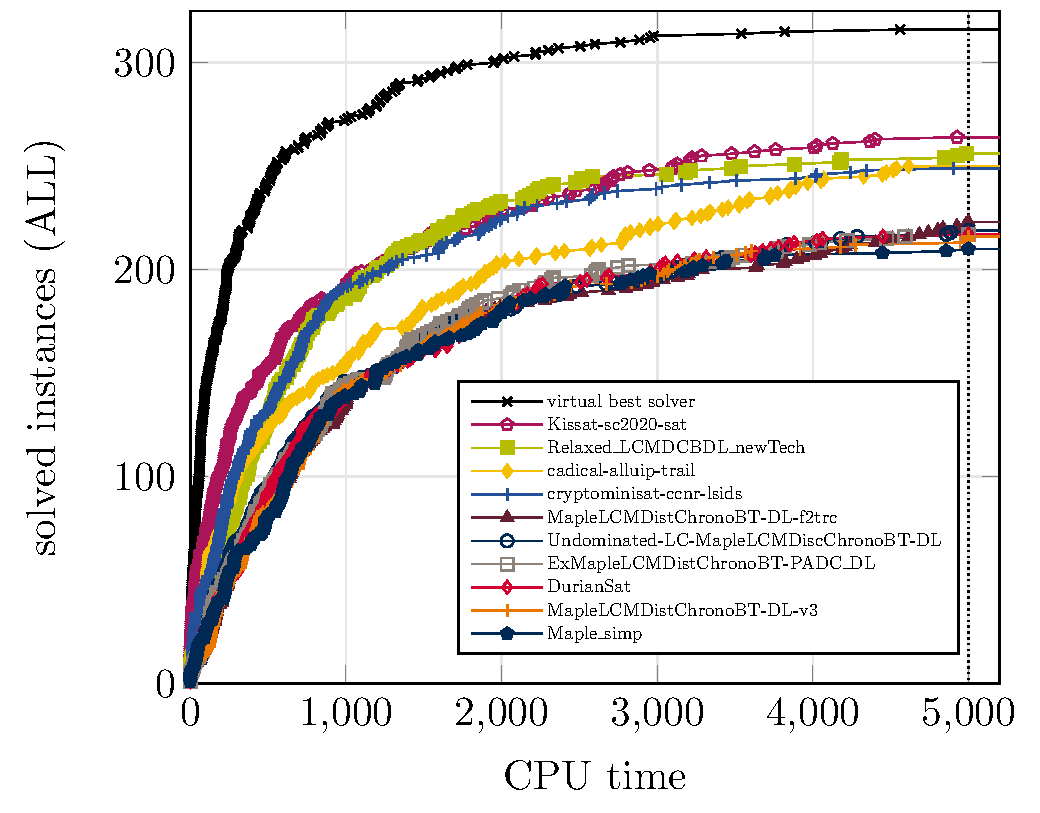
\includegraphics[width=.9\textwidth]{img/paper-main-top10-ALL.pdf}
\caption{Performance of the top 10 solvers + VBS on all  Main track benchmarks}
\label{main:all}
\end{figure}


The main reason for the separation between the top four solvers and the others is the enormous gap on satisfiable benchmarks, 
see Figure~\ref{main:sat}. In recent years, several techniques have been added to SAT solvers to improve
their performance on satisfiable instance. Examples of such techniques are the integration of a local search
solver and alternating between a SAT mode (infrequent restarts) and an UNSAT mode (frequent restarts,
and variable-move-to-front). The 2020 winner of the Main SAT track is \solver{Relaxed-newTech}, followed by 
\solver{Kissat-sat} and \solver{CMS-ccnr-lsids}.

\begin{figure}[ht]
\centering
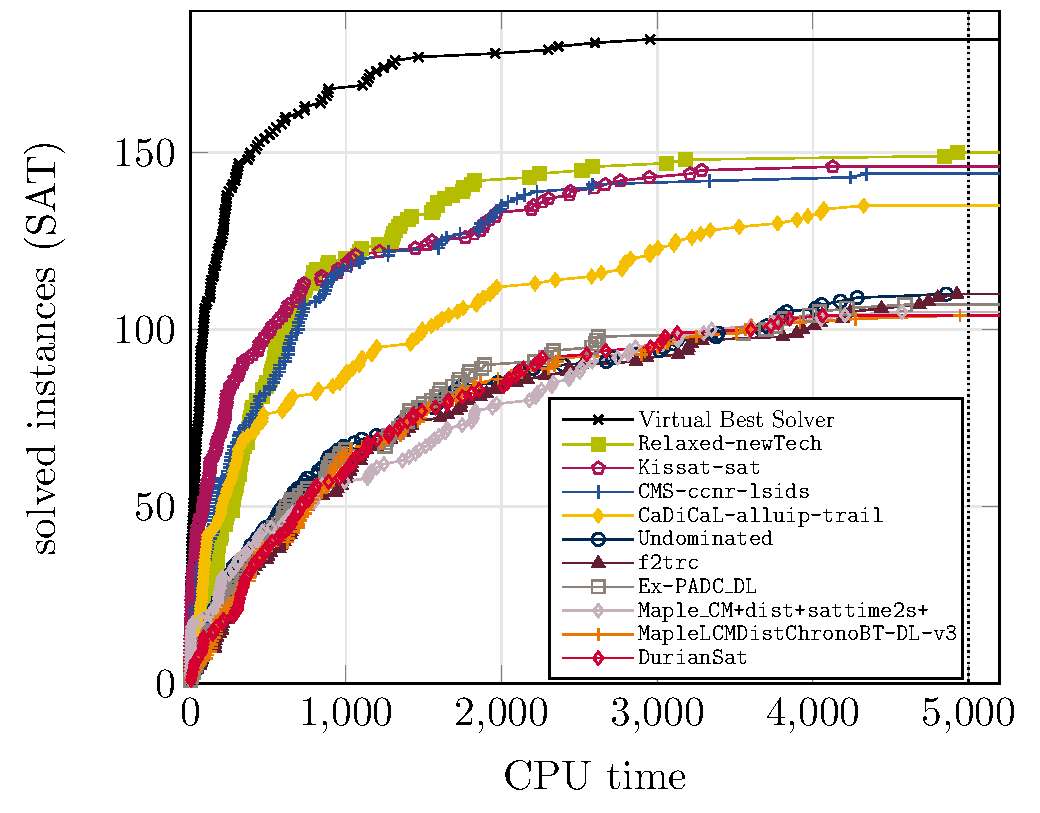
\includegraphics[width=.9\textwidth]{img/paper-main-top10-SAT.pdf}
\caption{Performance of the top 10 solvers + VBS on Main track satisfiable benchmarks}
\label{main:sat}
\end{figure}


The solver performances on unsatisfiable formulas was much closer,
see Figure~\ref{main:unsat}. Only \solver{Kissat-unsat}, the winner of the Main UNSAT track, 
performed significantly better compared to all other participants. It is therefore not surprising
that the VBS is reasonably close to \solver{Kissat-unsat}. \solver{Kissat} is a new solver that has been implemented in C, while most solvers are implemented in C++. Further 
details about \solver{Kissat} are described in Section~\ref{sec:kissat}.
The solvers \solver{CaDiCaL-trial}
and \solver{f2trc-s} won the second, respectively, third place in the Main UNSAT track.

\begin{figure}[ht]
\centering
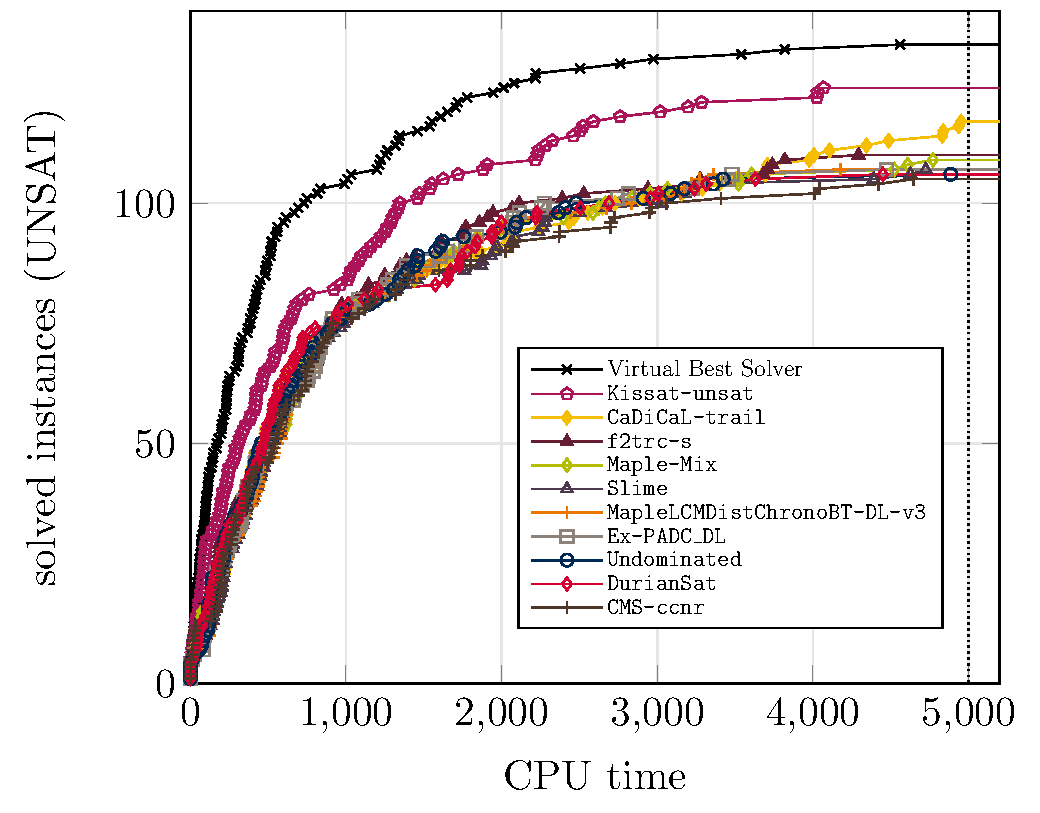
\includegraphics[width=.9\textwidth]{img/paper-main-top10-UNSAT.pdf}
\caption{Performance of the top 10 solvers + VBS on Main track unsatisfiable benchmarks}
\end{figure}
\label{main:unsat}

The ranking in the Planning Track was closer. \solver{CaDiCaL-alliup-trial}, the winning solver, 
solved only one instance more compared to the runner up \solver{CMS-ccnr-lsids}. Their PAR-2 score is 
quite close as well. The third ranked solver, \solver{Kissat}, solved fewer instances, but fast runtime
on several instances resulted in a strong PAR-2 score. Notice that these solvers were also strong in the Main tracks. 
Apparently none of the participating solvers was optimized for planning instances. 

The winning solver in the Parallel track is \solver{Painless-MCOMSPS-STR32}. The number in the postfix denotes
that this solver used 32 threads on the 64 virtual cores that were available. It has been observed in earlier 
competitions that uses fewer threads than the number of virtual cores can be helpful as threads compete 
for memory, which can reduce of the overall performance. The runner up is \solver{Plingeling}, while the
third place is for \solver{ManyGlucose-32}. Figure~\ref{fig:res-parallel} shows the performance of
all participating parallel solvers. Notice in Table~\ref{tab:results} that only the \solver{Painless-MCOMSPS-STR} solvers
and \solver{Plingeling} had a lower PAR-2 score than the winner of the Main Track (\solver{Kissat-sat}). 
This shows that it is hard to beat sequential solvers with a parallel solver on the competition instances. 
We will show later in the article (Table~\ref{tab:tuples}) that small sequential portfolios 
perform better (in terms of PAR-2 score) than the parallel solvers. 

\begin{figure}[ht]
\centering
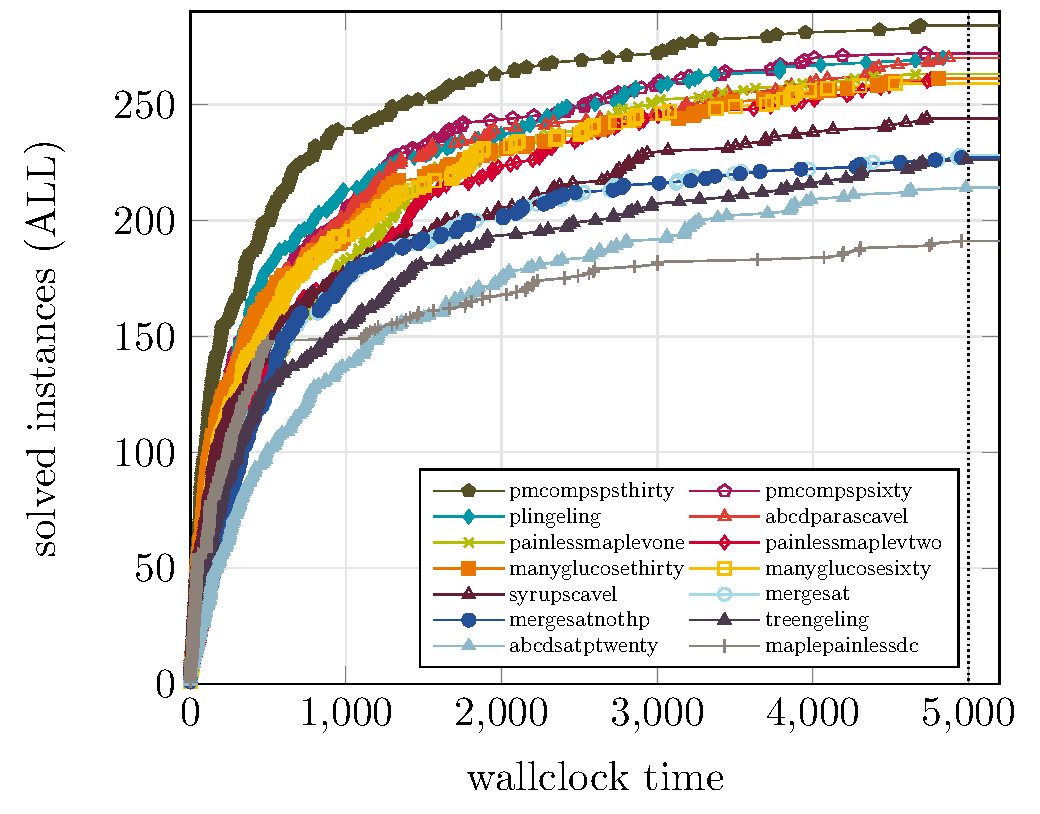
\includegraphics[width=.9\textwidth]{img/parallel-ALL.pdf}
\caption{Performance of the solvers in the Parallel track.}
\label{fig:res-parallel}
\end{figure}

The clear winner of the Cloud track is \solver{Mallob-Mono} and the runner-up is \solver{TopoSAT2},
see Figure~\ref{fig:res-cloud}.
\solver{Mallob-Mono} was able to solver more instances in 1000 seconds, compared to the 
winner of the Parallel Track in 5000 seconds, thereby showing the potential of distributed SAT solving. 
The other four participants performed significantly worse. This is likley due to the initial challenges
to develop a distributed solver. This was the first year of this track. We expect that the gap will be 
closer is future years. 


\begin{figure}
\centering
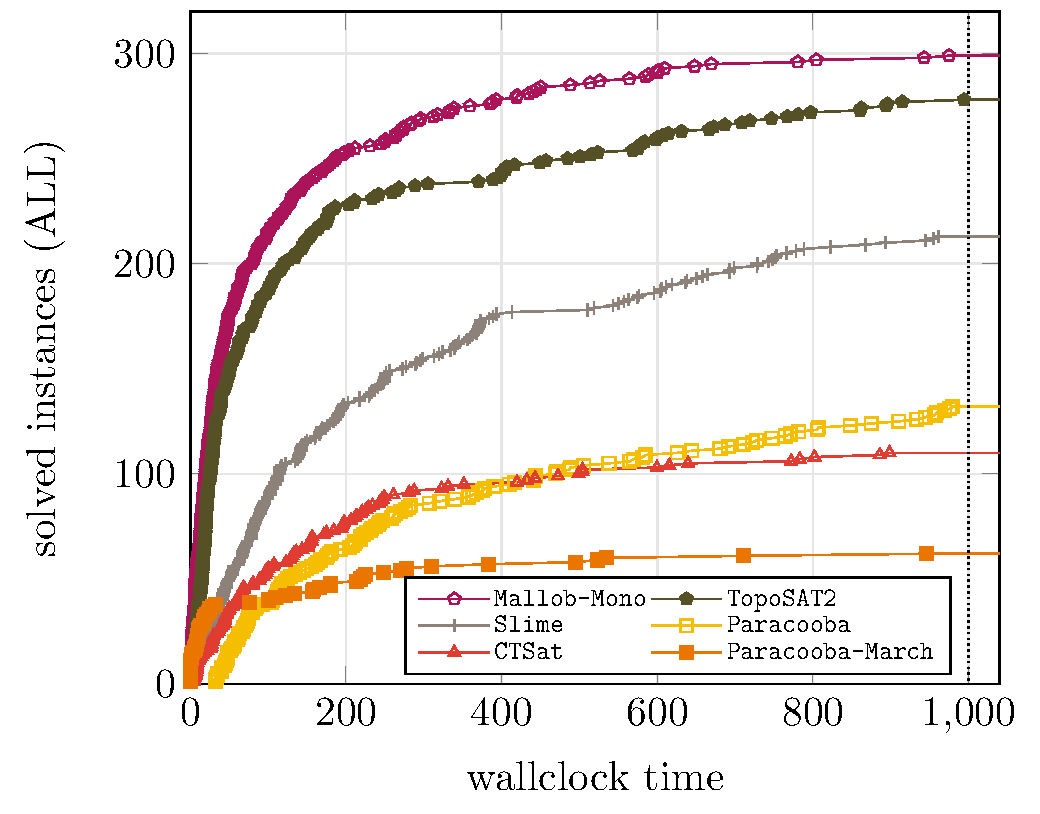
\includegraphics[width=.9\textwidth]{img/cloud-ALL.pdf}
\caption{Performance of the solvers in the Cloud track.}
\label{fig:res-cloud}
\end{figure}

\begin{table}
\centering\smaller
\setlength\tabcolsep{3pt}
%\begin{tabularx}{\linewidth}{X} \hline \end{tabularx}
\begin{tabularx}{.47\linewidth}{cccX}
\multicolumn{4}{l}{\bf Main Track}\\
\bf Pl. & \bf PAR-2 & \bf \# & \bf Solver \\
\arrayrulecolor{lightgray}\hline
1     & 3926.2 & 264 & \solbert{Kissat-sat} \\
(1)   & 4083.1 & 260 & \solver{Kissat} \\
2     & 4179.3 & 253 & \solbert{Relaxed-newTech} \\
3     & 4266.7 & 248 & \solbert{CMS-ccnr-lsids} \\
(3)   & 4278.0 & 250 & \solver{CMS-ccnr} \\
      & 4428.1 & 250 & \solver{CaDiCaL-alluip-trail} \\
      & 4429.6 & 250 & \solver{CaDiCaL-alluip} \\
      & 4436.5 & 245 & \solver{Relaxed} \\
      & 4501.2 & 243 & \solver{CMS-walksat} \\
      & 4554.0 & 243 & \solver{CaDiCaL-trail}%
%      & 4560.0 & 238 & \solver{Kissat-unsat} \\
%      & 4607.6 & 246 & \solver{CaDiCaL-sc2020} \\
%      & 5157.7 & 216 & \solver{Undominated} \\
%      & 5159.6 & 220 & \solver{f2trc-DL} \\
%      & 5177.0 & 214 & \solver{PADC-DL} \\  
\end{tabularx}\quad%
\begin{tabularx}{.5\linewidth}{cccX}
\multicolumn{4}{l}{\bf Parallel Track}\\
\bf Pl. & \bf PAR-2 & \bf \# & \bf Solver \\
\arrayrulecolor{lightgray}\hline
 1 & 3316.6 & 283 & \solbert{Painless-MCOMSPS-str32} \\
(1)& 3714.7 & 271 & \solver{Painless-MCOMSPS-str64} \\
 2 & 3743.4 & 269 & \solbert{Plingeling} \\
 3 & 3985.3 & 260 & \solbert{ManyGlucose-32} \\
   & 4022.7 & 262 & \solver{Painless-Maple-v1} \\
   & 4036.3 & 258 & \solver{ManyGlucose-64} \\
   & 4103.3 & 260 & \solver{Painless-Maple-v2} \\
   & 4433.3 & 243 & \solver{Syrup-Scavel} \\
   & 4903.4 & 225 & \solver{Treengeling} \\
   & 5240.1 & 213 & \solver{abcdsat-p20} \\
\end{tabularx}
~\\[1em]
\begin{tabularx}{.47\linewidth}{cccX}
\multicolumn{4}{l}{\bf Main Track, Satisfiable Instances}\\
\bf Pl. & \bf PAR-2 & \bf \# & \bf Solver \\
\arrayrulecolor{lightgray}\hline  
 1    & 2997.4 & 150 & \solbert{Relaxed-newTech} \\
 2    & 3127.6 & 146 & \solbert{Kissat-sat} \\
 3    & 3263.0 & 144 & \solbert{CMS-ccnr-lsids} \\
(3)   & 3317.4 & 145 & \solver{CMS-ccnr} \\
      & 3355.5 & 143 & \solver{Relaxed} \\
      & 3721.2 & 139 & \solver{CMS-walksat} \\
      & 3830.5 & 134 & \solver{Kissat} \\
      & 3908.5 & 135 & \solver{CaDiCaL-alluip-trail} \\
      & 3909.6 & 135 & \solver{CaDiCaL-alluip} \\
      & 4265.6 & 126 & \solver{CaDiCaL-trail}%
%      & 4368.6 & 130 & \solver{CaDiCaL-sc2020} \\
%   & 4804.9 & 114 & \solver{Kissat-unsat} \\
%   & 5173.2 & 110 & \solver{Undominated} \\
%   & 5244.1 & 107 & \solver{PADC-DL} \\
%   & 5264.9 & 110 & \solver{f2trc-DL} \\           
\end{tabularx}\quad%
\begin{tabularx}{.5\linewidth}{cccX}
\multicolumn{4}{l}{\bf Parallel Track, Satisfiable Instances}\\
\bf Pl. & \bf PAR-2 & \bf \# & \bf Solver \\
\arrayrulecolor{lightgray}\hline
 1 & 2853.7 & 153 & \solbert{Painless-MCOMSPS-str32} \\
 2 & 2913.6 & 154 & \solbert{Painless-Maple-v1} \\
(2)& 3082.7 & 151 & \solver{Painless-Maple-v2} \\
-- & 3196.9 & 148 & \solver{Painless-MCOMSPS-str64} \\
 3 & 3805.9 & 133 & \solbert{Plingeling} \\
   & 4048.3 & 130 & \solver{ManyGlucose-64} \\
   & 4076.2 & 130 & \solver{ManyGlucose-32} \\
   & 4675.4 & 119 & \solver{Syrup-Scavel} \\
   & 4907.1 & 114 & \solver{Treengeling} \\
   & 6337.5 & \phantom{0}85 & \solver{abcdsat-p20} \\
\end{tabularx}
~\\[1em]
\begin{tabularx}{.47\linewidth}{cccX}
\multicolumn{4}{l}{\bf Main Track, Unsatisfiable Instances}\\
\bf Pl. & \bf PAR-2 & \bf \# & \bf Solver \\
\arrayrulecolor{lightgray}\hline   
1     & 4315.1 & 124 & \solbert{Kissat-unsat} \\
(1)   & 4335.6 & 126 & \solver{Kissat} \\
(1)   & 4724.8 & 118 & \solver{Kissat-sat} \\
 2    & 4842.5 & 117 & \solbert{CaDiCaL-trail} \\
--    & 4846.7 & 116 & \solver{CaDiCaL-sc2020} \\
(2)   & 4947.8 & 115 & \solver{CaDiCaL-alluip-trail} \\
(2)   & 4949.6 & 115 & \solver{CaDiCaL-alluip} \\
 3    & 4991.4 & 110 & \solbert{f2trc-s} \\
(3)   & 5051.4 & 109 & \solver{f2trc} \\
(3)   & 5054.3 & 110 & \solver{f2trc-DL}%
%      & 5069.6 & 109 & \solver{Maple-Mix} \\
%      & 5110.0 & 107 & \solver{PADC-DL} \\
%      & 5126.9 & 107 & \solver{Maple-Simp} \\
%      & 5128.9 & 107 & \solver{MapleCBT-DL-v3} \\
%      & 5142.2 & 106 & \solver{Undominated} \\  
\end{tabularx}\quad%
\begin{tabularx}{.5\linewidth}{cccX}
\multicolumn{4}{l}{\bf Parallel Track, Unsatisfiable Instances}\\
\bf Pl. & \bf PAR-2 & \bf \# & \bf Solver \\
\arrayrulecolor{lightgray}\hline
 1 & 3680.8 & 136 & \solbert{Plingeling} \\
 2 & 3779.5 & 130 & \solbert{Painless-MCOMSPS-str32} \\
 3 & 3894.3 & 130 & \solbert{ManyGlucose-32} \\
(3)& 4024.2 & 128 & \solver{ManyGlucose-64} \\
   & 4142.8 & 128 & \solver{abcdsat-p20} \\
   & 4191.1 & 124 & \solver{Syrup-Scavel} \\
   & 4232.5 & 123 & \solver{Painless-MCOMSPS-str64} \\
   & 4899.8 & 111 & \solver{Treengeling} \\
   & 5123.9 & 109 & \solver{Painless-Maple-v2} \\
   & 5131.9 & 108 & \solver{Painless-Maple-v1}%
\end{tabularx}
~\\[1em]
\begin{tabularx}{.47\linewidth}{cccX}
\multicolumn{4}{l}{\bf Planning Track}\\
\bf Pl. & \bf PAR-2 & \bf \# & \bf Solver \\
\arrayrulecolor{lightgray}\hline   
 1    & 6406.9 & 80 & \solbert{CaDiCaL-alluip-trail} \\
(1)   & 6409.3 & 80 & \solver{CaDiCaL-alluip} \\
 2    & 6466.9 & 79 & \solbert{CMS-ccnr-lsids} \\
(2)   & 6471.9 & 79 & \solver{CMS-ccnr} \\
(2)   & 6472.9 & 79 & \solver{CMS-walksat} \\
 3    & 6596.4 & 75 & \solbert{Kissat-unsat} \\
      & 6650.1 & 79 & \solver{CaDiCaL-trail} \\
      & 6713.0 & 75 & \solver{Maple-Mix} \\
      & 6746.5 & 75 & \solver{MapleCOMSPS-init} \\
      & 6754.3 & 73 & \solver{Maple-Simp}%
%      & 6773.0 & 73 & \solver{MapleCOMSPS-drup} \\
%      & 6773.9 & 73 & \solver{Kissat-sat} \\
%      & 6774.2 & 73 & \solver{Kissat} \\
%      & 7025.5 & 68 & \solver{upGlucose3.0-PADC} \\
%      & 7044.7 & 66 & \solver{Glucose3.0-proofs} \\
\end{tabularx}\quad%
\begin{tabularx}{.5\linewidth}{cccX}
\arrayrulecolor{lightgray}
\multicolumn{4}{l}{\bf Cloud Track}\\
%\hline
\bf Pl. & \bf PAR-2 & \bf \# & \bf Solver \\
\hline
 1 & 2603.8 & 299 & \solbert{Mallob-Mono} \\
 2 & 3146.8 & 278 & \solbert{TopoSAT 2} \\
 3 & 4797.6 & 213 & \solbert{Slime} \\
   & 6800.8 & 132 & \solver{Paracooba} \\
   & 7299.0 & 110 & \solver{CTsat} \\
   & 8468.3 & \phantom{0}62 & \solver{Paracooba-March} \\
\phantom{0} & \phantom{0} & \phantom{0} & \phantom{0}\\
\phantom{0} & \phantom{0} & \phantom{0} & \phantom{0}\\
\phantom{0} & \phantom{0} & \phantom{0} & \phantom{0}\\
\phantom{0} & \phantom{0} & \phantom{0} & \phantom{0}
\end{tabularx}
\caption{Top 10 Solvers in Main, Planning, Parallel and Cloud Tracks: Place~(Pl.), Score (PAR-2) and Number of Solved Instances~(\#) per Solver}
\label{tab:results}
\end{table}


\section{Code-Bases and Winning Strategies}
\label{sec:analysis}

In the following, we provide an overview of the participating teams and solvers, 
and summarize new strategies which are implemented in the award winning solvers of this competition. 

We start with a few remarks on the evolution of code-bases of well known SAT solvers in Section~\ref{sec:codebases}. 
Our review of the winning strategies in this competition starts with sequential (including incremental) SAT solving in Section~\ref{sec:part:seq}, then we continue with parallel SAT solving in Section~\ref{sec:part:par} and conclude with solvers in the cloud track in Section~\ref{sec:part:cloud}. 


\subsection{Code-Bases of SAT Solvers: ``On the Shoulders of Giants''}
\label{sec:codebases}

Progress in SAT solvers is often based on successful modifications of existing code-bases. 
One well-known tree of development is rooted in the code-base of \solver{Minisat} by Eén and Sörenson~\cite{Niklas:2003:Minisat}. 
A well-known fork of \solver{Minisat} is \solver{Glucose} by Audemard and Simon~\cite{Audemard:2018:Glucose}, among others introducing Literal Block Distance (LBD) for weighing clauses in forgetting heuristics~\cite{Audemard:2009:Glucose}. 
The SAT solver \solver{RISS} by Manthey is a successful and award winning fork of \solver{Glucose} in combination with the state-of-the-art preprocessor \solver{Coprocessor}~\cite{Manthey:2012:Coprocessor2}. 

Another more recent string of development is rooted in the \solver{CoMinisatPS} fork of \solver{Minisat} by Chanseok Oh introducing three-tier clause-management~\cite{Oh:2015:satunsat}. 
The SAT solver \solver{Maple} appeared as a series of forks presenting innovative branching heuristics at SAT Competition 2016~\cite{Liang:2016:LRB}. 
The then award winning variant \solver{MapleCOMSPS} by Liang et al. is an implementation of a hybrid branching heuristic of classic Variable-State Independent Decaying Sum (VSIDS) and the new Learning-Rate based Branching (LRB) in \solver{CoMinisatPS}~\cite{Liang:2016:MapleCOMSPS}. 

In SAT Competition 2017, Luo et al. integrated learnt clause minimization based on unit propagation (\solver{LCM}) in their award winning \solver{Maple\_LCM\_Dist}~\cite{Luo:2017:LCM} which also uses the new branching heuristic \solver{Distance (Dist)} in an initial solving period~\cite{Xiao:2017:MapleLCMDist}. 
Using \solver{Maple\_LCM\_Dist}, Ryvchin and Nadel successfully integrated conditional chronological backtracking (\solver{ChronoBT})~\cite{Nadel:2018:CBT}. 
They presented their award winning \solver{Maple\_LCM\_Dist\_ChronoBT} in SAT Competition~2018~\cite{Ryvchin:SC2018:MapleChronoBT}. 

Kochemazov et al. improved three-tier clause-management by persisting
additional clauses through hash-based detection of repeatedly learned clauses and presented their award winning~\solver{MapleLCMDistChronoBT-DL} in SAT Race~2019~\cite{Kochemazov:SC2019:MapleChronoBTDL}. 
As can be seen in Table~\ref{tab:solvers-incremental}, numerous submissions to SAT Competition~2020 are forks of some recently award winning descendants of \solver{Maple}-based solver. 

Starting as a fork of \solver{Minisat} and the integration of special xor treatment~\cite{Soos:2009:Crypto}, \solver{CryptoMinisat} by Soos continues to be a state-of-the-art and feature-rich SAT solver. 
One highlight of \solver{CryptoMinisat} is its advanced data-logging capabilities for statistical analysis of SAT solver behavior~\cite{Soos:2019:ChrystalBall}.

Many independent and award-winning code-bases can be found among the SAT solvers written by Biere. 
The sequential SAT solver \solver{Lingeling} has been award winning since SAT Competition~2011 and is still competitive in its parallel version \solver{Plingeling}~\cite{Biere:2012:Lingeling}. 
As of SAT Competition~2017, \solver{CaDiCaL} % \cite{Biere:SC2020} - or cite some older proceedings to match the "As of SAT Competition~2017" part?
by Biere is another independent, award winning and structured implementation of the state-of-the-art in SAT solving. 
Its improved reimplementation \solver{Kissat}~\cite{Biere:SC2020} won in several of this competitions sequential tracks by a large margin. 

The sequential variant of the \emph{new code-base} \solver{ParaFrost} by Osama and Wijs was submitted for the first time in this competition and introduced several interesting new concepts~\cite{Osama:SC2020:Parafrost}. 


\subsection{Sequential SAT Solving}
\label{sec:part:seq}

Sequential SAT solvers have been evaluated in the Main, Planning and Incremental Library track of SAT Competition~2020. 
A total of $18$ teams submitted correct solvers to the Main track of the competition. 
Table~\ref{tab:solvers-main} displays an overview of the participating teams, base solvers and their variants. 
The recent genealogy of all submissions is highlighted by \emph{base solver} and \emph{variant} columns. 
Underlined text is used to point out the important parts of the respective submissions name.

\begin{table}[h!]
\setlength\tabcolsep{4.5pt}%default: 6pt
%\renewcommand{\arraystretch}{1.03}%default: 1
\smaller
\centering
\begin{tabularx}{\linewidth}{Xllcccc}
\bf Team & \bf Base Solver & \bf Variant / Name & \bf M & \bf U & \bf S & \bf P \\
\hline
\arrayrulecolor{lightgray}

\multirow{3}{*}{Biere} & \multirow{3}{*}{\solbert{Kissat}} &  -- & 1 & 1 & -- & --\\
 &  &  \solver{sat} & 1 & 1 & 2 & --\\
 &  &  \solver{unsat} & -- & 1 & -- & 3\\
\hline
 Biere, Fleury &  \solver{Cadical} & \solbert{SC2020} & -- & -- & -- & --\\
\hline
 
\multirow{2}{*}{Zhang, Cai}
    & \multirow{2}{*}{\solver{MapleLCMDistCBT-DL}} & \solbert{Relaxed} & -- & -- & -- & --\\
% &  & \solver{Rel. noTimeParam} & \\
 &  & \solver{Rel. newTech} & 2 & -- & 1 & --\\
\hline

\multirow{2}{*}{\stack{Soos, Cai, Devriendt, }{Gocht, Shaw, Meel}}~
 &  \multirow{2}{*}{\solver{CryptoMiniSat-CCAnr}} &  -- & 3 & -- & 3 & 2\\
 &  &  \solver{lsids} & 3 & -- & 3 & 2\\
\hline

\stack{Soos, Selman, Kautz, }{Devriendt, Gocht}~ & \solver{CryptoMiniSat-WalkSAT} & -- & -- & -- & -- & --\\
\hline

\multirow{4}{*}{\stack{Hickey, Feng, }{Bacchus}}
 &  &  \solver{trail} & -- & 2 & -- & --\\
 &  &  \solver{alluip} & -- & 2 & -- & 1\\
 & \multirow{-3}{*}{\solver{CaDiCaL}} &  \solbert{alluip-trail} & -- & 2 & -- & 1\\
 \cline{2-7}
 & \solver{MapleLCMDist} & \solver{alluip-trail} & -- & -- & -- & -- \\
\hline

\multirow{3}{*}{Kochemazov} & \multirow{2}{*}{\solver{MapleLCMDistCBT}} & \solbert{f2trc} & -- & 3 & -- & --\\
 & & \solver{f2trc-s} & -- & 3 & -- & --\\
 \cline{2-7}
 & \solver{MapleLCMDistCBT-DL} & \solver{f2trc} & -- & 3 & -- & --\\
\hline

\stack{Kochemazov, Zaikin, }{Kondratiev, Semenov} ~& \solbert{MapleLCMDistCBT-DL-v3} & -- & -- & -- & -- & -- \\
\hline

\multirow{4}{*}{\stack{Lonlac, }{Nguifo}}
 & \multirow{4}{*}{\solver{MapleLCMDistCBT-DL-v3}} & \solbert{Undominated} & -- & -- & -- & -- \\
 &  & \solver{Undom. Top16} & -- & -- & -- & -- \\
 &  & \solver{Undom. Top24} & -- & -- & -- & -- \\
 &  & \solver{Undom. Top36} & -- & -- & -- & -- \\
\hline

\multirow{4}{*}{\stack{Tchinda, }{Djamegni}}
 & \multirow{4}{*}{\solbert{Ex}\solver{MapleLCMDistCBT}} & \solver{padc\_dl} & -- & -- & -- & -- \\
 &  & \solver{padc\_dl\_ovau\_lin} & -- & -- & -- & -- \\
 &  & \solver{padc\_dl\_ovau\_exp} & -- & -- & -- & -- \\
 &  & \solver{psids\_dl} & -- & -- & -- & -- \\
% \cline{2-3}& Glucose 3.0 & upGlucose-3.0\_PADC\\
\hline

Shaw, Meel & \solver{MapleLCMDistCBT-DL-v3} & \solbert{DurianSat} & -- & -- & -- & -- \\
\hline

\multirow{2}{*}{Chen}
 & \multirow{2}{*}{\solver{MapleLCMDistCBT-DL}} & \solbert{Maple\_Mix} & -- & -- & -- & -- \\
 &  & \solbert{Maple\_Simp} & -- & -- & -- & -- \\
\hline

Riveros & \solver{MapleLCMDistCBT} & \solbert{SLIME} & -- & -- & -- & -- \\
\hline

\multirow{3}{*}{Li, Wu, Xu, Chen}
 & \multirow{3}{*}{\solver{MapleLCMDistCBT-DL}} & \solbert{Scavel} & -- & -- & -- & -- \\
 &  & \solver{Scavel01} & -- & -- & -- & -- \\
 &  & \solver{Scavel02} & -- & -- & -- & -- \\
\hline

\multirow{2}{*}{\stack{Liang, Oh, Nejati, }{Poupart, Ganesh}}
 & \multirow{2}{*}{\solbert{MapleCOMSPS\_LRB\_VSIDS\_2}} & -- & -- & -- & -- & -- \\
 &  & \solver{init} & -- & -- & -- & -- \\
\hline

\multirow{4}{*}{\stack{Chowdhury, }{Müller, You}}
 & \multirow{4}{*}{\solver{MapleLCMDistCBT-DL-v2.2}} & \solbert{exp}\solver{-V-LGB} & -- & -- & -- & -- \\
 &  & \solver{exp-V-L} & -- & -- & -- & -- \\
 &  & \solver{exp-L} & -- & -- & -- & -- \\
 &  & \solver{exp-V} & -- & -- & -- & -- \\
\hline

\multirow{4}{*}{\stack{Li, Luo, Xiao, }{Li, Manyà, Lü}}
 & \multirow{4}{*}{\solbert{MapleCM}} & \solbert{+dist} & -- & -- & -- & -- \\
 &  & \solver{+dist+sattime2s+-} & -- & -- & -- & -- \\
 &  & \solver{+dist+simp2--} & -- & -- & -- & -- \\
 &  & \solver{used+dist} & -- & -- & -- & -- \\
\hline

Kaiser, Hartung & \solver{MapleLCMDist} & \solbert{PauSat} & -- & -- & -- & -- \\
\hline

\multirow{2}{*}{Osama, Wijs} 
 & \multirow{2}{*}{\solbert{ParaFROST}} & -- & -- & -- & -- & -- \\
 &  & \solver{CBT} & -- & -- & -- & -- 
\end{tabularx}
\caption[Teams and Solvers in the Main Tracks]{\emph{Teams} and \emph{Solvers} in the Main Tracks. \emph{Base Solver} highlights solver genealogy while \emph{Variant} displays names of configurations and forks. Distinctive names are \solbert{underlined}. The rightmost columns indicate the awards given in the Main (\emph{M}) and Planning track (\emph{P}), and for performance on unsatisfiable (\emph{U}) and satisfiable (\emph{S}) instances.}
\label{tab:solvers-main}
\end{table}


%%%%%%%%%%%%%%%%%%%%%%%%%%%%%%%%%%%%%%%%%%%%%%%%%%

Four submissions made it to participate in the Incremental Library track, some of which, e.g, \solver{CryptoMiniSat-5}, have also been evaluated and awarded in the Main track. 
Submissions to the Incremental Library track have been evaluated with respect to $6$ different applications -- each with $50$ benchmark instances. 
Table~\ref{tab:solvers-incremental} displays an overview of the participating teams and solvers. 
In this table, \emph{Score} denotes the number of application categories in which the solvers won based on their PAR-2 score. 

\begin{table}[ht]
\centering\small
\begin{tabular}{llc}
\bf Team & \bf Solver & \bf Place\\
\hline
Soos, Cai, Devriendt, Gocht, Shaw, Meel & \solver{CryptoMiniSat 5} & 1 \\
Biere, Fleury & \solver{CaDiCaL 2020} & -- \\
Chen & \solver{abcdsat-i20} & -- \\
Manthey & \solver{Riss 7.1.2} & -- 
\end{tabular}
\caption[Teams and Solvers in the Incremental Track]{Teams and Solvers in the Incremental Library Track.}
\label{tab:solvers-incremental}
\end{table}


\subsubsection{Kissat} 
\label{sec:kissat}

Three configurations of \solver{Kissat} were evaluated in this competition, including one default configuration and two specialized configurations which are specifically tailored towards satisfiable and unsatisfiable instances, respectively. 
\solver{Kissat} received \emph{four awards}, by achieving first place in the Main track, best score on unsatisfiable instances, second best score on satisfiable instances and third place in the Planning track. 

\solver{Kissat} is a low-level reimplementation of \solver{CaDiCaL} with new sophisticated lazy data-structures for clause state monitoring, e.g., through binary clause inlining, sentinel values and bit stuffing~\cite{Biere:SC2019,Biere:SC2020}. 
Moreover, forward subsumption for learned clauses is mostly replaced by vivification algorithms~\cite{ChuMinLi:2020:Vivification}. 

Since conflict-rate has been observed to be too unstable for the use-case, \solver{Kissat} uses the new unit ``ticks'', which is based on the approximate number of cache-line accesses, to measure the length of two alternating restart-modes~\cite{Biere:SC2020}. 

Furthermore, \solver{Kissat} exploits autarkies to account for saved phases. 
In order to keep valuable information of saved phases, before each rephasing step, \solver{Kissat} computes the largest autarky for the assignment implied by the current saved phases~\cite{Kiesl:2019:Autarkies}. 
As such an autarky might contain satisfying assignments which imply disconnected components, those variables are subject to subsequent variable elimination. 


\subsubsection{CryptoMiniSat}
\label{sec:cryptominisat}

\solver{CryptoMiniSat} received \emph{four awards}, first place in the Incremental Library track, second place in the Planning track, third place in the Main track, and third best score on satisfiable instances. 
Two submitted variants \solver{default} and \solver{LSIDS} scored mostly adjacent ranks in the evaluation of tracks. 
The \solver{LSIDS} variant of \solver{CryptoMiniSat} comes with a new hybrid phase selection approach~\cite{Shaw:2020:LSIDS,Soos:SC2020}.

\solver{CryptoMiniSat} comes with an independent implementation of state-of-the-art hybrid branching heuristics which alternate between classic phase saving and target phase selection~\cite{Biere:SC2019}.
\solver{CryptoMiniSat-CCAnr} regularly schedules short periods of local search and imports the best assignment for phase selection -- a procedure which is known as ``rephasing'' from CaDiCaL~\cite{Biere:SC2019}.
In addition, \solver{CryptoMiniSat-CCAnr} bumps the VSIDS scores of the first 100 variables in those clauses which the SLS solver weighs most hard to satisfy~\cite{Soos:SC2020}.

Inprocessing has been extended to include ternary resolution and more vivification~\cite{ChuMinLi:2020:Vivification}. 
\solver{CryptoMinisat} alternates decay factors of its branching heuristics, thus avoiding the restriction to a ``single best'' configuration~\cite{Soos:SC2020}. 
The submitted version of \solver{CryptoMinisat} entails a new optimized implementation of Gauss-Jordan Elimination~\cite{Soos:2020:CNFXOR}. 
\solver{CryptoMinisat} periodically executes the \solver{BreakId} algorithm to  calculate symmetry breaking clauses~\cite{Devriendt:2016:BreakId}.


\subsubsection{CaDiCaL AllUip}

Based on \solver{CaDiCaL}, its variants \solver{Trail} and \solver{AllUip} present implementations of a new \emph{Trail Saving} approach~\cite{Hickey:2020:TrailSaving} and improved clause-learning \emph{Stable AllUIP}~\cite{Bacchus:SC2020}. 
Submitted were the three variants \solver{Trail}, \solver{AllUip} and \solver{AllUip+Trail}. 
The variants including \emph{Stable AllUIP} were the most successful and won the first price in the Planning track. 

\emph{Stable AllUip} resolves additional clauses beyond the 1st Unit Implication Point (1-UIP) and keeps them if they are of smaller size or LBD than the 1-UIP clause. 
By monitoring the frequency of clauses which successfully pass that filter, the solver dynamically limits the amount of such extended learning attempts~\cite{Zhang:2001:ClauseLearning,Bacchus:SC2020}.
The \emph{Trail Saving} variant caches backtracked portions of the trail and uses them to restore decision levels during search if possible~\cite{Hickey:2020:TrailSaving}. 


\subsubsection{Relaxed newTech}

The \solver{Relaxed} fork of \solver{MapleLCMDistCBT-DL} was first presented in SAT Race 2019~\cite{Xindi:SC2019}. 
In SAT Competition~2020, its variant \solver{newTech} showed a good performance especially on satisfiable instances. 
The solver achieved two awards, the second price in the Main track and the best score on satisfiable instances. 

\solver{Relaxed} integrates short runs of the local search solver \solver{CCAnr} through periodic export and import of assignments~\cite{Xindi:SC2019} and uses a probabilistic schedule for switching between $10$ phase selection modes. 
The \solver{Relaxed newTech} variant uses occurrence counts of variables in unsatisfied clauses during SLS runs to recalculate variable priorities for their modified branching heuristic~\cite{Xindi:SC2020}. 


\subsubsection{Maple F2TRC}

The \solver{F2TRC} fork of \solver{MapleLCMDistCBT} achieved the third best score on unsatisfiable instances. 
\solver{F2TRC} comes with deterministic reimplementations of former winning strategies in \solver{Maple}, e.g., by replacing time-based intervals through conflict-based intervals~\cite{Kochemazov:SC2020}. 

\solver{F2TRC} introduces improved management of learned clauses in the tree tiers \emph{core}, \emph{tier2} and \emph{local} which are inherited from \solver{CoMinisatPS}~\cite{Oh:2015:satunsat}.
A dynamic size limit for the \emph{core} tier triggers the reassignment of inactive clauses from \emph{core} to \emph{tier2}. 
To counter-act an observed starving of tier2, the conflict-based heuristic that controls demotion of clauses from \emph{tier2} to \emph{local} was replaced by a size based heuristic~\cite{Kochemazov:SC2020}. 


\subsection{Parallel SAT Solving: Winners of the Parallel Track}
\label{sec:part:par}

\begin{table}[b]
\centering\small
\begin{tabular}{llccc}
\bf Team & \bf Solver & \bf U+S & \bf U & \bf S \\
\hline\arrayrulecolor{lightgray}
\multirow{2}{*}{\stack{Vallade, Le Frioux, Baarir, }{Sopena, Kordon}}~
 & \solver{Painless-MCOMSPS-STR-32} & 1 & 2 & 1 \\
 & \solver{Painless-MCOMSPS-STR-64} & 1 & --& --\\
\hline
\multirow{2}{*}{Biere, Fazekas, Heisinger}
 & \solver{Plingeling} & 2 & 1 & 3 \\
 & \solver{Treengeling} & --& --& --\\
\hline
\multirow{2}{*}{Nabeshima, Inoue}
 & \solver{ManyGlucose-32} & 3 & 3 & -- \\
 & \solver{ManyGlucose-64} & -- & 3 & --\\
\hline
\multirow{2}{*}{Tchinda, Djamegni}
 & \solver{Painless-Maple-v1} & --& --& 2 \\
 & \solver{Painless-Maple-v2} & --& --& 2 \\
\hline
Li, Wu, Xu, Chen & \solver{Syrup Scavel} & --& --& --\\
%\hline
Chen & \solver{abcdSAT-p20} & --& --& --
\end{tabular}
\caption{Teams and Solvers participating in the Parallel track.}
\end{table}


\subsubsection{Painless MapleCOMSPS STR} 

\solver{Painless-MCOMSPS-STR} integrates the solver \solver{MapleCOMSPS} in the \solver{Painless} parallelization framework~\cite{Frioux:2017:Painless,Liang:2017:Maplecomsps}. 
The authors submitted a \solver{32} and a \solver{64} threaded variant and won three awards: first place overall, best score on satisfiable and second best score on unsatisfiable instances. 
In the overall evaluation, the \solver{32} threaded variant achieved slightly better scores than the \solver{64} threaded variant. 
However, in the separate evaluations on satisfiable and unsatisfiable variants the \solver{32} threaded variants performed much better, such that the runner-up solvers outperformed the \solver{64} threaded variant. 

\solver{Painless} uses a generic interface to integrate a solver and abstracts away the implementation details of parallelism and concurrent data-structures, such that implementations in \solver{Painless} boil down to implementing parallelization and clause sharing strategies~\cite{Frioux:2017:Painless}. 

\solver{Painless-MCOMSPS-STR} diversifies mainly via hard-coded configurations of the branching strategies LRB and VSIDS, and via sparse random initialization of variable polarities~\cite{Balyo:2015:HordeSATs}. 
Two special solver instances perform concurrent clause strengthening~\cite{Wieringa:2013:CCS} Gaussian elimination, respectively. 
\solver{Painless-MCOMSPS-STR} uses an all-to-all strategy for clause sharing with a fixed size clause buffer and an LBD filter with a dynamic limit~\cite{SC2020}. 


\subsubsection{Plingeling} 

\solver{Plingeling} achieved the best score on unsatisfiable instances, second place in the overall evaluation, and the third best score on satisfiable instances. 
\solver{Plingeling} is built around the well-known \solver{Lingeling} and did not change since 2016. 
In a global master queue, \solver{Plingeling} shares unit clauses, equivalences and short clauses with a size limit of~$40$ and an LBD limit of~$8$. 
\solver{Plingeling} uses random seeds for diversification via variable polarities~\cite{Biere:SC2020,Biere:2012:Lingeling}. 


\subsubsection{ManyGlucose}

\solver{ManyGlucose} was submitted in \solver{32} and \solver{64} threaded variants. 
The \solver{32} threaded variant received two awards in this competition: the overall third place and third best score on unsatisfiable instances. 
\solver{ManyGlucose} is a fork of \solver{GlucoseSyrup} that uses strategies known from \solver{ManySat} to achieve deterministic solver behaviour~\cite{Audemard:2018:GlucoseSyrup}~\cite{Audemard:2014:LazyClauseExchange}~\cite{Hamadi:2009:ManySat}. 


\subsubsection{Painless Maple} 

\solver{Painless Maple} received the award for the second best performance on satisfiable instances but had the worst performance on unsatisfiable instances. 
\solver{Painless Maple} integrates the solver \solver{ExMapleLCMDistChronoBT} into the \solver{Painless} parallelization framework~\cite{Frioux:2017:Painless}. 
\solver{Painless Maple} uses a sharing strategy in which the solvers are divided into those which only export clauses and others which import \emph{and} export clauses. 
\solver{Painless Maple} was submitted in two variants \solver{v1} and \solver{v2}. 
\solver{Painless Maple v1} diversifies via hand-crafted heuristic configurations and \solver{Painless Maple v2} diversifies via randomized intialization of branching heuristics~\cite{SC2020}. 


\subsection{Massively Parallel SAT Solving: Winners of the Cloud Track}
\label{sec:part:cloud}

\begin{table}[t]
\centering\small
\begin{tabular}{llc}
\bf Team & \bf Solver & \bf Place\\
\hline\arrayrulecolor{lightgray}
Schreiber & \solver{Mallob Mono} & 1\\
Ehlers, Kulczynski, Nowotka, Sieweck & \solver{TopoSAT 2} & 2\\
Riveros & \solver{Slime} & 3\\
\hline
\multirow{2}{*}{Biere, Fazekas, Fleury, Heisinger} & \solver{Paracooba}, & --\\
& \solver{Paracooba-March} & --\\
\hline
Hartung & \solver{CTSat} & --
\end{tabular}
\caption{Teams and solvers participating in the Cloud track.}
\end{table}


\subsubsection{Mallob Mono}

\solver{Mallob} is a fork of the generic massively parallel SAT solver \solver{HordeSAT}~\cite{Balyo:2015:HordeSATs}. 
\solver{Mallob} performs dynamic load balancing through \emph{malleable job scheduling} in case the input contains several SAT instances of varying priorty. 
This functionality is disabled in the submitted variant \solver{Mallob Mono}. 
\solver{Mallob} uses \solver{Lingeling-bcj} and as every 14th solver \solver{Mallob} spawns the SLS solver \solver{YalSAT}~\cite{Biere:2018:LingelingYalsat}.
Diversification is done via randomized sparse initialization of branching scores. 

\solver{Mallob} shares clauses by organizing solvers in a binary tree in which clauses are asynchronously aggregated in a buffer which is passed along this tree from its leafs to the root. 
Each node performs a three-way merge of its local export buffer and the two incoming buffers. 
The aggregate that approaches the root of the binary tree is then broadcast to all solvers~\cite{Schreiber:SC2020}. 

\solver{Mallob} uses a global clause size limit and a dynamic size limit for the sharing buffer, which depends on its position in the binary tree and is larger the closer we get to the root. 
Clauses are sorted by their size during aggregation, such that smaller clauses are preferred over longer clauses. 
Duplicates are avoided by using a bloom filter which is cleared periodically~\cite{Schreiber:SC2020}. 


\subsubsection{TopoSAT 2}

\solver{TopoSAT~2} is a massively parallel SAT solver using \solver{Glucose~3}~\cite{Audemard:2018:Glucose}~\cite{Ehlers:2018:Toposat2}. 
\solver{TopoSAT~2} uses lock-free clause-exchange for solvers on the same machine, and Message Passing Interface (MPI) to share clauses between machines~\cite{Hamadi:2009:ManySat}. 
\solver{TopoSAT~2} strengthens clauses before export and delays clause import until the trail-size reaches a local minimum. 
\solver{Toposat~2} diversifies via strategies used for branching, restarting and clause forgetting~\cite{Ehlers:SC2020}. 


\subsubsection{Slime}

\solver{Slime} is built from \solver{MapleLCMDistChronoBT} and was first submitted as a sequential solver to SAT Race~2019 with a new phase selection heuristic~\cite{Riveros:SC2019}. 
The new submitted version of \solver{Slime} comes with periodic randomization in geometrically increasing intervals~\cite{Riveros:SC2020}. 
Even thought its sequential version was unsuccessful in the Main track, the MPI-based cloud version of \solver{Slime} won the third price in the Cloud track. 


\section{Differentiated Analysis of Main Track Results}

In this section, we provide additional views on the Main track results,
focusing on metrics complementing the PAR-2 score, 
which we used for ranking the solvers in the actual competition.

\subsection{Contributions to the Virtual Best Solver}

The Virtual Best Solver (VBS) is a fictitious solver consisting 
of all the solvers that actually participated in the competition (or a specific track)
and an oracle which, when given an input instance,
invokes to run the actual solver which performed the best on that instance.
In this way, the performance of the VBS highlights a certain upper bound 
on performance achievable in principle by the technology 
of the participating solvers (cf.~the figures in Section~\ref{sec:results}). 

One can see that the VBS solves all the instances that
were solved by at least one solver and solves each instance in the best observed time.
By quantifying how much each participating solver contributes
to the performance of the VBS, we may attempt to establish which
technology (as represented by the solvers) is the most important
(and to what degree) in the observed state of the art of SAT solving.
We came up with the following three related metrics conceptually derived
from the notion of VBS:
\begin{description}
\item[VBS1]
``The fastest takes it all'':
For each solver we count the number of times, it was the fastest to solve an instance.
\item[VBS2]
``Time aware, but proportional'':
A solver $S$ solving an instance $I$ in time $T^S_I$ accrues 
the following fraction of a point for solving $I$:
$T^\mathit{VBS}_I/T^S_I$, where $T^\mathit{VBS}_I$ is the solution time of the best solver on $I$.
\item[VBS3]
``Split the point for solving'':
We award each solver $S$ solving an instance $I$ the fraction $1/|\mathcal{S}_I|$ of points, where
$\mathcal{S}_I$ is the set of solvers solving $I$.
\end{description}
We remark that the sum of VBS1 points, as well as VBS3 points, computed across all the solvers
is equal to the number of instances solved by at least one solver (later denoted \emph{total}).
This is obvious for VBS1, as exactly one solver scores a point for solving an instance.
In the case of VBS3, where we discard the information about the solution times, 
we evenly split the one point reward for solving an instance to those solvers which were successful on it.

In contrast, VBS2 does not have this property as it in general distributes more than one point per instance.
Similarly to VBS1, it takes the solution time into account,
and similarly to VBS3 it does not award just the best solver on an instance.
For example, being twice as slow on an instance than the fastest solver results in a half point awarded.
And, if all the solvers solve an instance with the same solution time,
each solver scores a whole point for that instance. 

\begin{table}
%\setlength\tabcolsep{1.5pt}
\smaller
%\centering
\begin{tabular}{ccl}
\bf VBS-1 & \bf \% & \bf Solver \\
\hline
46 & 11.5 & \solver{Kissat-unsat} \\
39 & \phantom{0}9.8 & \solver{Kissat-sat} \\
26 & \phantom{0}6.5 & \solver{Kissat} \\
18 & \phantom{0}4.5 & \solver{CMS-ccnr-lsids} \\
14 & \phantom{0}3.5 & \solver{MapleCM+dist+sat2s} \\
13 & \phantom{0}3.2 & \solver{Relaxed} \\
13 & \phantom{0}3.2 & \solver{Maple-alluip-tr.} \\
12 & \phantom{0}3.0 & \solver{upGlucose3.0-PADC} \\
10 & \phantom{0}2.5 & \solver{CMS-ccnr} \\
10 & \phantom{0}2.5 & \solver{CaDiCaL-sc2020} \\
\end{tabular}\qquad%
%~\\[1em]
\begin{tabular}{ccl}
\bf VBS-2 & \bf \% & \bf Solver \\
\hline
131.5 & 32.9 & \solver{Kissat-sat} \\
122.6 & 30.6 & \solver{Kissat} \\
115.4 & 28.9 & \solver{Kissat-unsat} \\
\phantom{0}92.3 & 23.1 & \solver{CMS-ccnr-lsids} \\
\phantom{0}88.8 & 22.2 & \solver{CMS-ccnr} \\
\phantom{0}84.1 & 21.0 & \solver{CaDiCaL-alluip-tr.} \\
\phantom{0}84.0 & 21.0 & \solver{CaDiCaL-alluip} \\
\phantom{0}83.0 & 20.7 & \solver{CaDiCaL-sc2020} \\
\phantom{0}82.3 & 20.6 & \solver{Relaxed-newTech} \\
\phantom{0}81.5 & 20.4 & \solver{Relaxed} \\
\end{tabular}%
~\\[1em]
\begin{tabular}{ccl}
\bf VBS-3 & \bf \% & \bf Solver \\
\hline
13.0 & 3.3 & \solver{Kissat} \\
11.9 & 3.0 & \solver{Kissat-unsat} \\
11.7 & 2.9 & \solver{Relaxed-newTech} \\
11.4 & 2.8 & \solver{Kissat-sat} \\
10.8 & 2.7 & \solver{CaDiCaL-alluip-tr.} \\
10.8 & 2.7 & \solver{CaDiCaL-alluip} \\
10.5 & 2.6 & \solver{Relaxed} \\
10.4 & 2.6 & \solver{CaDiCaL-sc2020} \\
10.3 & 2.6 & \solver{CMS-walksat} \\
\phantom{0}9.6 & 2.4 & \solver{CaDiCaL-trail} \\
\end{tabular}
\caption{VBS metrics for the results of the Main track, all instances. 
The total number of solved problems was 316. 
There were 48 (non-disqualified) solvers (and their configurations).
Each table shows the first ten solvers sorted according to the respective metric.}
\label{tab:vbsMainALL}
\end{table}

%\begin{table}
%\caption{VBS metrics for the results of the Main track, SAT instances. 
%The total number of solved problems was 182. 
%There were 48 (non-disqualified) participating solvers.
%Each table always shows the first ten solvers sorted according to the respective metric.}
%\label{tab:vbsMainSAT}
%\begin{center}
%\begin{tabular}{ccl}
%VBS1 & percent total & solver \\
%\hline
%29 & 15.9 & Kissat-sat \\
%16 & \phantom{0}8.8 & Kissat \\
%14 & \phantom{0}7.7 & MapleCM+dist+sat2s \\
%12 & \phantom{0}6.6 & CMS-ccnr-lsids \\
%10 & \phantom{0}5.5 & Relaxed \\
%\phantom{0}8 & \phantom{0}4.4 & CMS-ccnr \\
%\phantom{0}8 & \phantom{0}4.4 & CaDiCaL-sc2020 \\
%\phantom{0}8 & \phantom{0}4.4 & Kissat-unsat \\
%\phantom{0}6 & \phantom{0}3.3 & CaDiCaL-trail \\
%\phantom{0}5 & \phantom{0}2.7 & MapleCOMSPS\_drup \\
%\end{tabular}
%\end{center}
%\begin{center}
%\begin{tabular}{ccl}
%VBS2 & percent total & solver \\
%\hline
%70.1 & 38.5 & Kissat-sat \\
%48.6 & 26.7 & Kissat \\
%45.2 & 24.8 & CMS-ccnr-lsids \\
%43.4 & 23.8 & Relaxed\_newTech \\
%42.4 & 23.3 & CMS-ccnr \\
%41.6 & 22.8 & Relaxed \\
%34.7 & 19.0 & CaDiCaL-alluip-trail \\
%34.6 & 19.0 & CaDiCaL-alluip \\
%33.7 & 18.5 & CMS-walksat \\
%32.8 & 18.0 & CaDiCaL-sc2020 \\
%\end{tabular}
%\end{center}
%\begin{center}
%\begin{tabular}{ccl}
%VBS3 & percent total & solver \\
%\hline
%9.3 & 5.1 & Relaxed\_newTech \\
%8.1 & 4.4 & Relaxed \\
%7.8 & 4.3 & CMS-walksat \\
%7.0 & 3.8 & Kissat-sat \\
%6.7 & 3.7 & Kissat \\
%6.7 & 3.7 & CMS-ccnr \\
%6.6 & 3.6 & CMS-ccnr-lsids \\
%6.2 & 3.4 & CaDiCaL-sc2020 \\
%6.2 & 3.4 & CaDiCaL-alluip-trail \\
%6.2 & 3.4 & CaDiCaL-alluip \\
%\end{tabular}
%\end{center}
%\end{table}

%\begin{table}
%\caption{VBS metrics for the results of the Main track, UNSAT instances. 
%The total number of solved problems was 134. 
%There were 48 (non-disqualified) participating solvers.
%Each table always shows the first ten solvers sorted according to the respective metric.}
%\label{tab:vbsMainUNSAT}
%\begin{center}
%\begin{tabular}{ccl}
%VBS1 & percent total & solver \\
%\hline
%38 & 28.4 & Kissat-unsat \\
%11 & \phantom{0}8.2 & Maple-alluip-trail \\
%10 & \phantom{0}7.5 & Kissat \\
%10 & \phantom{0}7.5 & Kissat-sat \\
%\phantom{0}8 & \phantom{0}6.0 & MapleCMused+dist \\
%\phantom{0}7 & \phantom{0}5.2 & upGlucose3.0\_PADC \\
%\phantom{0}6 & \phantom{0}4.5 & CMS-ccnr-lsids \\
%\phantom{0}3 & \phantom{0}2.2 & f2trc \\
%\phantom{0}3 & \phantom{0}2.2 & Relaxed \\
%\phantom{0}3 & \phantom{0}2.2 & Glucose3.0\_proofs \\
%\end{tabular}
%\end{center}
%\begin{center}
%\begin{tabular}{ccl}
%VBS2 & percent total & solver \\
%\hline
%86.5 & 64.6 & Kissat-unsat \\
%74.0 & 55.2 & Kissat \\
%61.4 & 45.8 & Kissat-sat \\
%55.4 & 41.4 & f2trc-s \\
%55.2 & 41.2 & DurianSat \\
%53.6 & 40.0 & Maple-alluip-trail \\
%53.4 & 39.8 & f2trc \\
%52.4 & 39.1 & f2trc-DL \\
%51.8 & 38.6 & MapleCMused+dist \\
%51.7 & 38.6 & PADC\_DL \\
%\end{tabular}
%\end{center}
%\begin{center}
%\begin{tabular}{ccl}
%VBS3 & percent total & solver \\
%\hline
%6.7 & 5.0 & Kissat-unsat \\
%6.3 & 4.7 & Kissat \\
%4.7 & 3.5 & CaDiCaL-trail \\
%4.6 & 3.5 & CaDiCaL-alluip-trail \\
%4.6 & 3.5 & CaDiCaL-alluip \\
%4.4 & 3.3 & Kissat-sat \\
%4.3 & 3.2 & CaDiCaL-sc2020 \\
%3.5 & 2.6 & f2trc-s \\
%3.4 & 2.5 & exp\_V\_LGB\_MLD\_CBT\_DL \\
%3.1 & 2.3 & f2trc-DL \\
%\end{tabular}
%\end{center}
%\end{table}
%\todo{Probably hide tab:vbsMainSAT and tab:vbsMainUNSAT.} 

Table~\ref{tab:vbsMainALL} renders the just described three metrics applied 
to the full results of the Main track. We can see that the respective leaderboards 
are generally dominated by \solver{Kissat} and its configurations.
VBS1 tells us that \solver{Kissat-unsat} was most often the fastest solver,
in particular on \SI{11.5}{\percent} of all the solved instances.

VBS2 highlights as first \solver{Kissat-sat}. Its leading \SI{32.9}{\percent} of total is a bit harder to 
interpret: A solver can score \SI{32.9}{\percent} of VBS2 total
by solving \SI{32.9}{\percent} of the solved instances in the best observed time
and no others. But we know, thanks to its VBS1, that \solver{Kissat-sat} solved \SI{9.8}{\percent}
of the solved instances in the best observed time (and some others).
A solver can also score \SI{32.9}{\percent} of VBS2 total by solving all the solved instances,
but always being roughly 3 times slower than the VBS. 
\solver{Kissat-sat} lies obviously somewhere between these two extremes.

Finally, according to VBS3, the best solver is \solver{Kissat} with 13.0 points,
which amounts to \SI{3.3}{\percent} of the distributed total score.
The VBS3 metric is generally the most evenly distributed one,
at least among the first 10 solvers. 
(The last solver got 0.9 points which is \SI{0.221}{\percent} of the total.)
One can conclude from this that most of the benchmarks are solved
by most of the well performing solvers. 

\subsection{Greedy set cover}
Another perspective on how much each solver contributes to the state of the art
can be obtained by attempting to construct a sequential schedule of solvers 
(rather then relying on an oracle to pick one for each instance, as with VBS)
and looking at how big role each solvers plays in such a schedule. Since constructing 
an optimal schedule tends to be computationally hard, we start here by 
presenting a useful efficient alternative -- a greedy set cover approach.

With greedy set cover, we start with an empty schedule and iteratively consider 
each solver for the addition to the schedule obtained so far, picking the one
with the highest ``marginal contribution'' in terms of the number of problems
the new schedule will be able to solve. This is perhaps best demonstrated on
the actual data from the competition, again taking the Main track results. 

\begin{table}
\centering\small
\begin{tabularx}{\linewidth}{cXccc}
\bf Iteration & \bf Selected Solver & \bf Solved & \bf Contributes \\ % & covered so far \\
\hline\arrayrulecolor{lightgray}
\phantom{0}1 & \solver{Kissat-sat} & 264 & 264 \\ % & 264 \\
\phantom{0}2 & \solver{CaDiCaL-alluip} & 250 & \phantom{0}22 \\ % & 286 \\
\phantom{0}3 & \solver{f2trc-s} & 214 & \phantom{0}10 \\ % & 296 \\
\phantom{0}4 & \solver{Relaxed-newTech} & 253 & \phantom{00}6 \\ % & 302 \\
\phantom{0}5 & \solver{Kissat-unsat} & 238 & \phantom{00}4 \\ % & 306 \\
\phantom{0}6 & \solver{Relaxed} & 245 & \phantom{00}3 \\ % & 309 \\
\phantom{0}7 & \solver{CMS-walksat} & 243 & \phantom{00}3 \\ % & 312 \\
\phantom{0}8 & \solver{CMS-ccnr-lsids} & 248 & \phantom{00}1 \\ % & 313 \\
\phantom{0}9 & \solver{MapleCBT-DL-v3} & 211 & \phantom{00}1 \\ % & 314 \\
10 & \solver{DurianSat} & 210 & \phantom{00}1 \\ % & 315 \\
11 & \solver{exp-V-LGB-MLD-CBT-DL} & 194 & \phantom{00}1 \\ % & 316 \\
\hline
 & Total & -- & 316 \\
\end{tabularx}
\caption{A greedy set cover of the solved instances by solvers of the Main track.}
\label{tab:gscMain}
\end{table}

A greedy set cover of the solved instances by solvers of the Main track is presented in Table~\ref{tab:gscMain}. 
In the first iteration, the solver which solved the highest number of instances is selected; in our case it was \solver{Kissat-sat} with 264 instances as we know already from Table~\ref{tab:results}.
Given those 264 instances as already covered, \solver{CaDiCaL-alluip} was the best in further contributing to the set by additional $22$ instances in iteration $2$.
We can see that the further iterations tend to add very little,
with the final four iterations adding one instance each. Note that each solver
that managed to solve an instance uniquely (i.e.~being the only solver to do so)
is showing up in the table. This is, for example the case of the last listed  
\solver{exp-V-LGB-MLD-CBT-DL}.
Highlighting unique solutions is a property of the greedy set cover metric
which we believe is congruent with documenting contributions to the state of the art.

\subsection{Time-limited schedules}

The greedy set cover technique focuses only on solving instances,
disregarding the time it would take to execute the obtained schedule. We can
also look at schedules that would fit in a prescribed time budget. A natural choice
of the budget seems to be the original time limit of \SI{5000}{\second}.

\begin{table}
\centering\small
\begin{tabulary}{\linewidth}{cccL}
\bf k & \bf Time (s) & \bf Solved & \bf Best Schedule \\
\hline
1 & 5000 & 264 & \{ \solver{Kissat-sat} \}\\
2 & 2500 & 278 & \{ \solver{Kissat-unsat}, \solver{Relaxed-newTech} \}\\
3 & 1666 & 272 & \{ \solver{Kissat-unsat}, \solver{Kissat-sat}, \solver{CMS-ccnr-lsids} \} \\
4 & 1250 & 262 & \{ \solver{Kissat-unsat}, \solver{Kissat-sat}, \solver{CMS-ccnr-lsids}, \phantom{\{ }\solver{Maple-alluip-trail} \}\\ 
5 & 1000 & 253 & \{ \solver{Kissat-unsat}, \solver{Kissat-sat}, \solver{CMS-ccnr-lsids}, \phantom{\{ }\solver{Maple-alluip-trail}, \solver{CaDiCaL-alluip} \}\\
\end{tabulary}
\caption{Schedules that maximize the number of solved Main track instances for $k \in \{1, \dots, 5\}$ solvers among which $5000$ seconds are split uniformly.}
\label{tab:MainUniformTimeSplit}
\end{table}

By employing a brute-force approach we first constructed a sequences of schedules 
where the $i$-th schedule splits the available time of \SI{5000}{\second} uniformly among
$i$ solvers and solves the highest number of instances under these constraints.
The results are presented in Table~\ref{tab:MainUniformTimeSplit}.
We can see that the initial increase from 264 to 278 of ``covered'' instances 
when using two solvers instead of one (although allowing each to only use half of the time)
does not continue further with additional solvers allowed,
although its still better to use three solvers in a fair time split 
(and cover 272 instances) than just one.
One could use this observation to conjecture that the really hard 
problems that were solved actually require quite a large time to 
get ``cracked'' by any solver and thus the advantage of adding more solvers to the schedule
quickly diminishes.

We complemented this ``uniform time split'' schedule by formulating the schedule construction
problem as a MaxSMT formula and using the Z3 SMT solver \cite{DBLP:conf/tacas/MouraB08} in its optimization mode \cite{DBLP:conf/sycss/BjornerP14} to solve it.
For each solver (and its configuration) $S$ we introduced an integer variable $R^S$ denoting 
the number of seconds $S$ will run in the new schedule. We then constructed a formula with the hard
constraints $0 \leq R^S$ for every $S$ and $\sum_{S\in\mathcal{S}} R^S \leq 5000$ and with one 
soft constraint for every instance $I$ of the form
\[\bigvee_{S \in \mathcal{S}_I} T^S_I \leq R^S,\]
where $\mathcal{S}_I$ is the set of solvers which solved the instance $I$ and $T^S_I$ is the time it took solver $S$ to solve $I$ here rounded up to the nearest integer.
(Note that while $R^S$ are variables, i.e.~unknowns, the $T^S_I$ are known constants in the formula.)

\begin{table}
\centering\small
\begin{tabularx}{\linewidth}{Xccc}
\bf Solver & \bf Time (s) & \bf Solved & \bf Contributes \\
\hline\arrayrulecolor{lightgray}
\solver{Kissat-unsat} & 2523 & 219 & 219 \\
\solver{Relaxed-newTech} & 2180 & 234 & \phantom{0}59 \\
\solver{Kissat-sat} & \phantom{0}103 & \phantom{0}72 & \phantom{00}2 \\
\solver{f2trc-DL} & \phantom{00}76 & \phantom{0}15 & \phantom{00}0 \\
\solver{CaDiCaL-alluip} & \phantom{00}58 & \phantom{0}26 & \phantom{00}2 \\
\solver{Maple-alluip-trail} & \phantom{00}34 & \phantom{0}12 & \phantom{00}1 \\
\solver{MapleCM+dist+sat2s} & \phantom{00}18 & \phantom{0}18 & \phantom{00}1 \\
\solver{CaDiCaL-sc2020} & \phantom{000}8 & \phantom{0}10 & \phantom{00}2 \\
\hline 
Total & 5000 & \phantom{0}-- & 286 \\ 
\end{tabularx}
\caption{An optimal \SI{5000}{\second} schedule for the Main track
constructed using Z3.}
\label{tab:MainZ3Schedule}
\end{table}

Finding a solution which satisfies all the hard constraints and as many soft constraints as possible,
Z3 came up with the schedule shown in Table~\ref{tab:MainZ3Schedule} (in under two hours on a single core of a \SI{2.30}{\giga\hertz} CPU).
The table is sorted by $R^S$, the time the schedule allocates to individual solvers, and skips the zero entries.
It is not clear to what degree is the obtained schedule unique and how much it relies on each solver being present and for how long.
Nevertheless, it is interesting to observe the total number of problems covered, here 286,
and compare it to the 278 achieved in Table~\ref{tab:MainUniformTimeSplit} with the uniform split and two solvers.

Amusingly, as can be seen from the ``contributes'' column, the presence of \solver{f2trc-DL} in the schedule is not necessary.
% The following three lines could be skipped without much harm:
All the 15 instances this solver solves under 76 seconds were already covered by the preceding three solvers.
This result, however, does not signify a bug, as Z3 was not asked to produce a schedule with a minimal number of
participating solvers.
Indeed, allowing any other solver to run for the 76 ``wasted'' seconds would not increase the overall total.


\subsection{Small Portfolios}

\begin{table}[t]
\centering\small
\begin{tabulary}{\linewidth}{rLl}
\bf k & \bf Best k-Tuple & \bf Score\\ 
\hline\arrayrulecolor{lightgray}
1 & \{ \solver{Kissat-sat} \} & $3926.2$\\
\hline
2 & \{ \solver{Kissat-unsat}, \solver{Relaxed-newTech} \} & $3160.5$\\
3 & \{ \solver{Kissat-unsat}, \solver{Relaxed-newTech}, \solver{CaDiCaL-2020} \} & $2986.4$\\
4 & \{ \solver{Kissat}, \solver{Relaxed-newTech}, \solver{CaDiCaL-2020}, \solver{Scavel01} \} & $2842.6$\\
5 & \{ \solver{Kissat-unsat}, \solver{Relaxed-newTech}, \solver{CaDiCaL-2020}, \solver{Scavel01}, \phantom{\{ }\solver{CMS-Walksat} \} & $2757.3$\\
6 & \{ \solver{Kissat-sat}, \solver{Kissat-unsat}, \solver{Relaxed}, \solver{Relaxed-newTech}, \phantom{\{ }\solver{CaDiCaL-alluip-trail}, \solver{f2trc-s} \} & $2687.0$\\
7 & \{ \solver{Kissat-sat}, \solver{Kissat-unsat}, \solver{Relaxed}, \solver{Relaxed-newTech}, \phantom{\{ }\solver{CaDiCaL-alluip-trail}, \solver{f2trc-s}, \solver{CMS-Walksat}\} & $2616.9$\\
\hline
48 & \emph{Set of all Solvers} & $2431.4$
\end{tabulary}
\caption{Best performing k-tuples in terms of their VBS's PAR-2 score.}
\label{tab:tuples}
\end{table}

The PAR-2 score of the VBS of all $48$ submitted solvers in the Main track is $2431.4$, which is close to 40\% better than the PAR-2 score of $3926.2$ of the single best solver \solver{Kissat-sat}. 
Given the set of solvers $S$, the set of tuples of size $k$ is defined as follows $P_k := \{ T \mid T \in 2^S \land |T| = k\}$.
We calculated the PAR-2 score for each VBS created from solver tuples in $P_k$. 
In Table~\ref{tab:tuples}, we report on the single best performing $k$-tuple $T_k \in P_k$ ($1 \leq k \leq 7$). 

Interestingly, each of the first five tuples $T_{k \leq 5}$ contains exactly one of the three \solver{Kissat} variants. 
For $i < 5$ the relation $T_{i} \subset T_{i+1}$ holds only under projection to base solvers due to the fluctuating variants of \solver{Kissat}. 
The composition changes more strongly in $T_6$. 
Interestingly, we now have both variants $\{ \solver{Kissat-sat}, \solver{Kissat-unsat} \} \subset T_6$, and moreover it holds that $T_6 \subset T_7$.
All solvers in $T_{k \leq 7}$ belong the top performing solvers which received an award in the Main track, with the only exception being $\solver{Scavel01} \in T_4 \cap T_5$ (cf.~Table~\ref{tab:results}). 


\subsection{Score per Instance Family} 

\begin{table}[b]
\small
\begin{tabularx}{\linewidth}{X|rrrrrr}
 & \multicolumn{2}{l}{\solver{Kissat-sat}} & \multicolumn{2}{l}{\solver{Relaxed-newTech}} & \multicolumn{2}{l}{\solver{CMS-ccnr-lsids}} \\
\bf Family & \bf Pl. & \bf PAR-2 & \bf Pl. & \bf PAR-2 & \bf Pl. & \bf PAR-2 \\
\hline
Anti-Bandwidth 			& 26 & 7435.6 &  2 & 5863.2 &  \bf 1 & 4958.7\\
Bit-Vector 				&  \bf 7 & 8310.2 & 22 & 8772.4 & 42 & 9005.9\\
Coloring 				&  \bf 2 & 5357.1 & 11 & 7589.3 & 13 & 7910.1\\
Core-Based Generator 	&  \bf 3 & 1217.0 & 29 & 3170.7 &  4 & 1253.3\\
Cryptography 			&  \bf 4 & 3451.4 &  6 & 3526.9 & 10 & 4124.2\\
Hypertree Decomposition & 21 & 1173.3 &  \bf 8 & 1016.0 & 38 & 3188.0\\
Influence Maximization 	& 22 & 2350.4 &  \bf 3 & 1838.9 & 11 & 2035.8\\
Tensors 				&  \bf 2 & 1412.4 &  7 & 4411.2 & 11 & 7414.2\\
Timetable 				& 41 & 7889.0 & 21 & 5103.8 & \bf 19 & 5092.4\\
Tournament 				& 4 & 10000.0&  \bf 2 & 8715.0 &  4 & 10000.0\\
Vlsat 					& 27 & 7149.7 &  5 & 5307.5 &  \bf 1 & 5026.4\\
\end{tabularx}
\caption{Place and PAR-2 of Winning Solvers in the Main Track per Instance Family}
\label{tab:eval-by-family}
\end{table}

Contributions to the VBS can be well capatured by clustering the instance space into instance families. 
We evaluated the runtimes of the three winning solvers of the Main track on those new families which are represented by at least $14$ instances (cf. Table~\ref{tab:families}) and report on their place and score in Table~\ref{tab:eval-by-family}. 
Interestingly, the overall winning solver \solver{Kissat-sat} is outperformed by the second and third ranked solvers \solver{Relaxed-newTech} and \solver{CMS-ccnr-lsids} on the \emph{Anti-Bandwidth}, \emph{Vlsat}, and \emph{Influence Maximization} families by a large margin. 

\subsection{Similarity of Solvers}
To investigate the similarity of solvers from the Main track, we define a
similarity metric based on measured runtimes. We start by removing $84$
benchmarks that have not been solved by any solver. For the rest, a PAR-2 score
is assigned to each instance for every solver,
% based on the \num{5000}-second timeout
\emph{i.e.}, we set a score of \num{10000} for unsolved instances.
Each solver $S$ thus is associated with the PAR-2 scores $S_{1},\dots,S_{316}$.
% This leaves us with $316$ floats
% $S_{1},\dots,S_{316}$ for each solver $S$.
The \emph{similarity} of two solvers $S$
and $S'$, normalized to the interval $[0,1]$ is defined
as:
% by Equation~\ref{eq-similarity}.

% \begin{equation}
% \label{eq-similarity}
\[
	similarity(S, S') =\quad 1 - \frac{\sum{|S_{i} - S'_{i}|}}{316 \cdot \num{10000}}
\]
% \end{equation}
We calculated the \emph{similarity} of the $30$ solvers with the
best average PAR-2 score in the Main track. The results are displayed in
Figure~\ref{fig-similarity-main} as a \emph{heat map}, similar to the visualization in \cite{Balyo:2015:SATRace}. Additionally, the result
of hierarchically clustering the solvers based on their similarity is
illustrated as a \emph{dendrogram}. The height at which two solvers or clusters
are joined reflects how similar they are. For example, enabling the \emph{trail
  saving} in \solver{CaDiCaL-alluip} has no impact on the runtime, resulting in
a similarity above \num{0.999}. Therefore the two solvers are joined low in the
dendrogram.
% A similar visualization was used for the results of the SAT Race 2015 \cite{Balyo:2015:SATRace}.

One big cluster that we identify consists of the \solver{Maple}-decedents,
all of which are modifications of the winners in the SAT Competition 2018 and
the SAT Race 2019.
The similarity within the cluster is high, with the exception of
\solver{Scavel} and \solver{exp\_V\_MLD\_CBT\_DL}.
They form a subcluster
with a lower similarity to the rest, but a high similarity within. In fact, the highest measured similarity,
 % of $0.96$
besides the aforementioned \solver{CaDiCaL-alluip}, is observed between them.
The two solvers are both based on
\solver{MapleLCMDistChronoBT-dl-v2.2} but have different authors.
The high similarity suggest that the
changes they made either result in a very similar behavior or do not have a
significant impact on the runtime performance.

The two configurations of \solver{Relaxed} by \emph{Zhang} and \emph{Cai}
use the same codebase as a lot of solvers in the Maple-Cluster but their
overall performance is better and closer to the \solver{CMS}-Cluster.
The three \solver{CMS} configurations
differ in their implementation of stochastic local search
(SLS) and have similar performance.
The 2020 version of \solver{CaDiCaL}
performed worse than the modifications based on the 2019 version and
does not quite fit into any cluster.

The last cluster to the left of the heat map is comprised of the other solvers
originally written by \emph{Biere}. Interesting to note is that the
\solver{Kissat} configuration specialized for unsatisfiable instances joins the
others in the cluster high in the dendrogram. In fact \solver{Kissat-unsat} has
the lowest average similarity to all other solvers in the top 30.
This suggests its importance for an optimal
portfolio.
% Average similarity
% | Kissat-unsat         |  21.75012381941168 |
% | Kissat               | 22.591060319234913 |
% | CaDiCaL-alluip       |  22.93588211785061 |
% | CaDiCaL-alluip-trail |  22.93631201417939 |
% | Kissat-sat           |  22.99738644487821 |

% The other sub-cluster consists of modifications to the 2019 version of
% \solver{CaDiCaL}.
% The new version CaDiCaL-2020 has a worse overall performance
% than the solvers in this cluster and a comparatively high similarty to the
% Maple-Cluster.

\begin{figure}[tp]
    \centering
    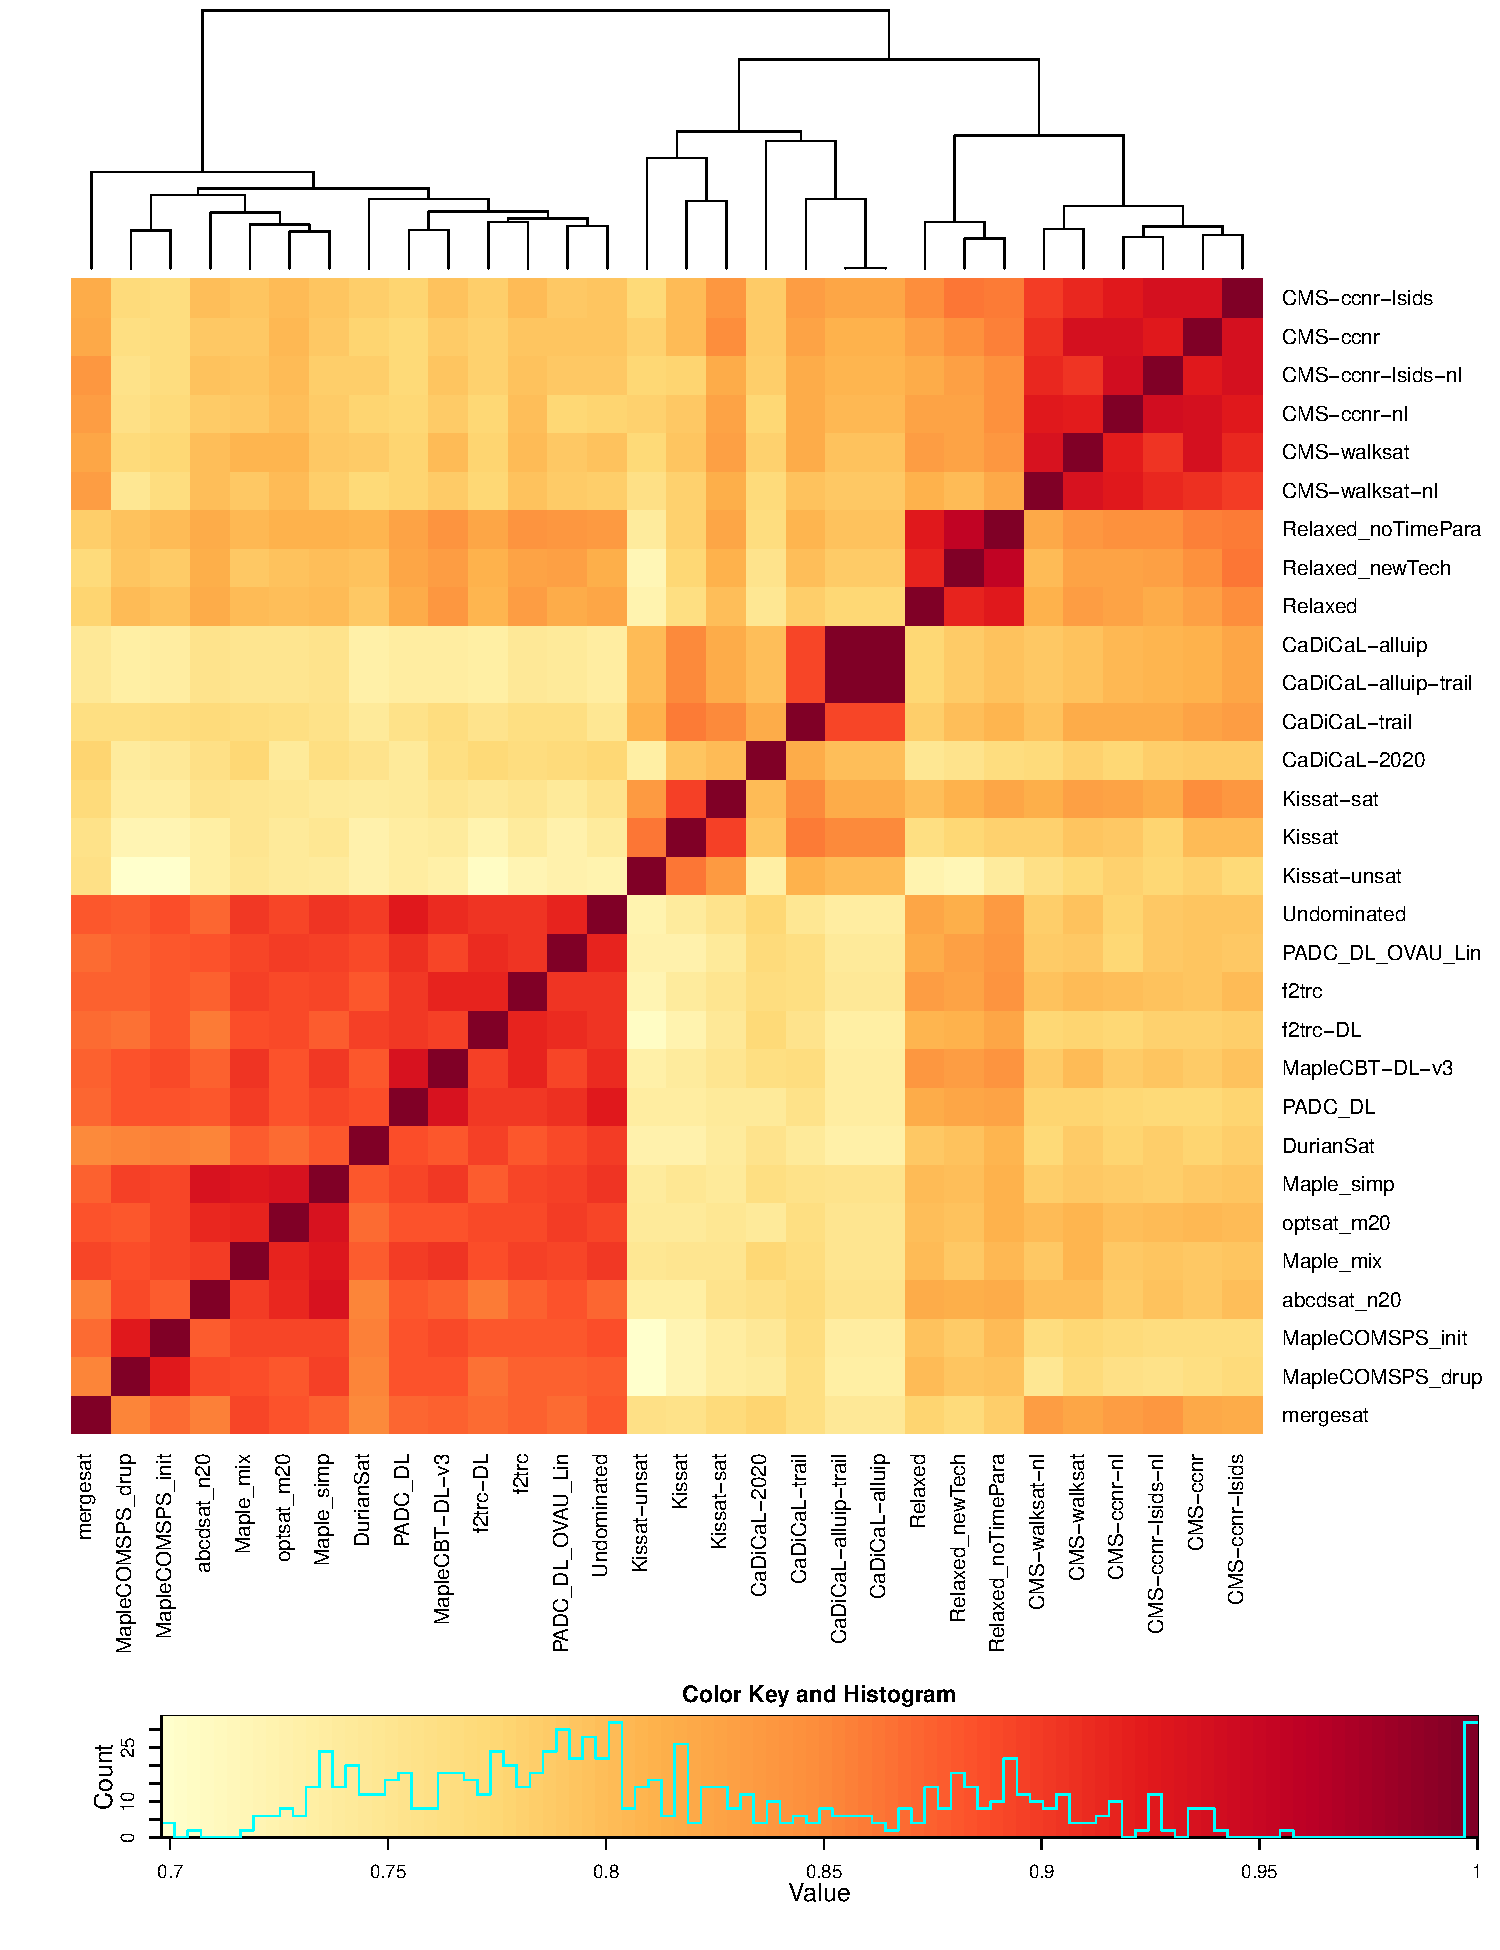
\includegraphics[width=\textwidth]{similarity/cross.pdf}
    \caption{Heat-map and dendrogram (top) based on the runtime similarity of the solvers participating in the Main track.
      Darker regions mean that the solvers are more similar.
      A more precise relation between color and similarity-value together with a histogram of the values that appear is given at the bottom.
    }
    \label{fig-similarity-main}
\end{figure}

% \subsection{Solver Ranking Robustness}
\subsection{Influence of Benchmark Selection on Solver Ranking}
The main result of the competition is the ranking of the solvers participating
in the Main track, according to their average PAR-2 score. To evaluate the impact
of benchmark selection on the solver ranking, we follow the experiments
described in the tool suite
\texttt{benchfeature}\cite{benchfeature}.
% \footnote{\url{http://fmv.jku.at/benchfeature/}} developed
% by Fazekas, Kaufmann and Biere.
% performed the following
% experiment:

We first use random sampling to select subsets of benchmarks used in the Main track.
We start with $316$ benchmarks that have been solved by at least one solver in
the Main track and remove a number of benchmarks randomly. For each
possible subset size (1--316) we generate 50 random samples.

The solvers are assigned a new rank in ascending order of their PAR-2 score on
each random sample. Note that we never encounter a tie. This ranking can be
seen as an estimate of the original ranking.
If even relatively small random samples result in a good estimate, we draw a
positive conclusion about the robustness of the ranking.
% We draw a positive conclusion about the robustness of the original ranking, if
% even the resulting estimate from relatively small random samples
% are good approximations.
To determine how similar an estimate is to the original ranking, we calculate
the \emph{Spearman's rank correlation coefficient} of the two rankings.
% and compute the correlation coefficient.

Spearman's rank correlation coefficient
for two rankings $r_{1}$ and $r_{2}$
is defined by the following equation:
% \begin{equation}
% \label{eq-spearman}
\[
    \rho = 1 - \frac{6\cdot\sum_{S}{(r_{1}(S) - r_{2}(S))^2}}{n(n^2-1)},
\]
% \end{equation}
where $n$ is the number of solvers in the Main track ($48$), and the rankings
$r_{\{1,2\}}(S)$ map a solver $S$ to its rank, \emph{i.e.,} $1$ for the best
performing solver, whereas $48$ is assigned to the solver
with the highest average PAR-2 score.

The coefficient $\rho$ is in the interval $[-1, 1]$, where a rank correlation of
$1$ means that the two rankings are equal and $-1$ means that one ranking is the
reverse of the other. To give a better intuition for $\rho$, we list a few
modifications to the original ranking together with the resulting rank
correlation coefficient. The smallest change we can make is to switch the rank
of two adjacent solvers, resulting in a high rank correlation $\rho = 0.9999$.
Several small changes also result in a high rank correlation; repeating the same
modification as before $n/2$ times to switch all pairs of adjacent solvers in
rank still gives a value of $\rho = 0.9974$. On the other hand, switching the
highest ranked solver (\solver{Kissat-sat}) with the lowest,
results in a rank correlation of $\rho = 0.7602$. Moving \solver{Kissat-sat} to
the bottom of the ranking while moving every other solver up one rank gives a
higher $\rho = 0.8776$. Doing the same to all three \solver{Kissat}
configurations (with ranks 1, 2 and 11, now 46, 47 and 48) results in
$\rho = 0.6839$.

The mean and standard deviation of the computed correlation coefficients are
depicted in Figure~\ref{fig:sampleAll}.
\begin{figure}[h]
  \label{fig:sampleAll}
  \centering
  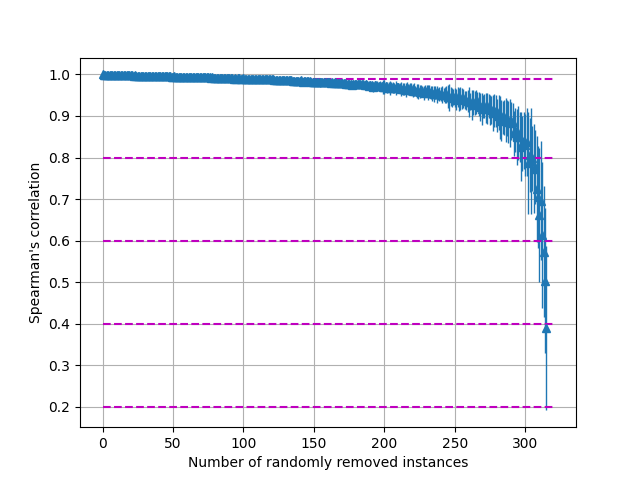
\includegraphics[width=0.8\textwidth]{stability/ALL_random_smpling_correlations.png}
  \caption{Mean and standard deviation of rank correlation under removal of random instances over 50 samples for each size}
\end{figure}
The rank correlation is high even for relatively small samples.
The average rank correlation drops below $0.99$ only after randomly removing at least $95$ benchmarks, which is $30\%$ of the considered benchmark set. Accordingly, removing fewer benchmarks randomly has almost no effect on the ranking of the solvers.
Furthermore, removing fewer than $200$ ($63\%$) benchmarks, still results in an average rank correlation above $0.96$.

This suggests that the impact of the random selection in Algorithm~\ref{algo:select} on the solver ranking is limited.
% \ref{sec:byob}
The collected data cannot show whether all of the benchmarks originally
submitted by the solver authors have a systematic bias. However, since each
newly submitted benchmark family originates from a different domain and is often
the result of current research, we can assume that the submitted families
together are representative.

\begin{figure}[h]
  \label{fig:sampleFamily}
  \centering
  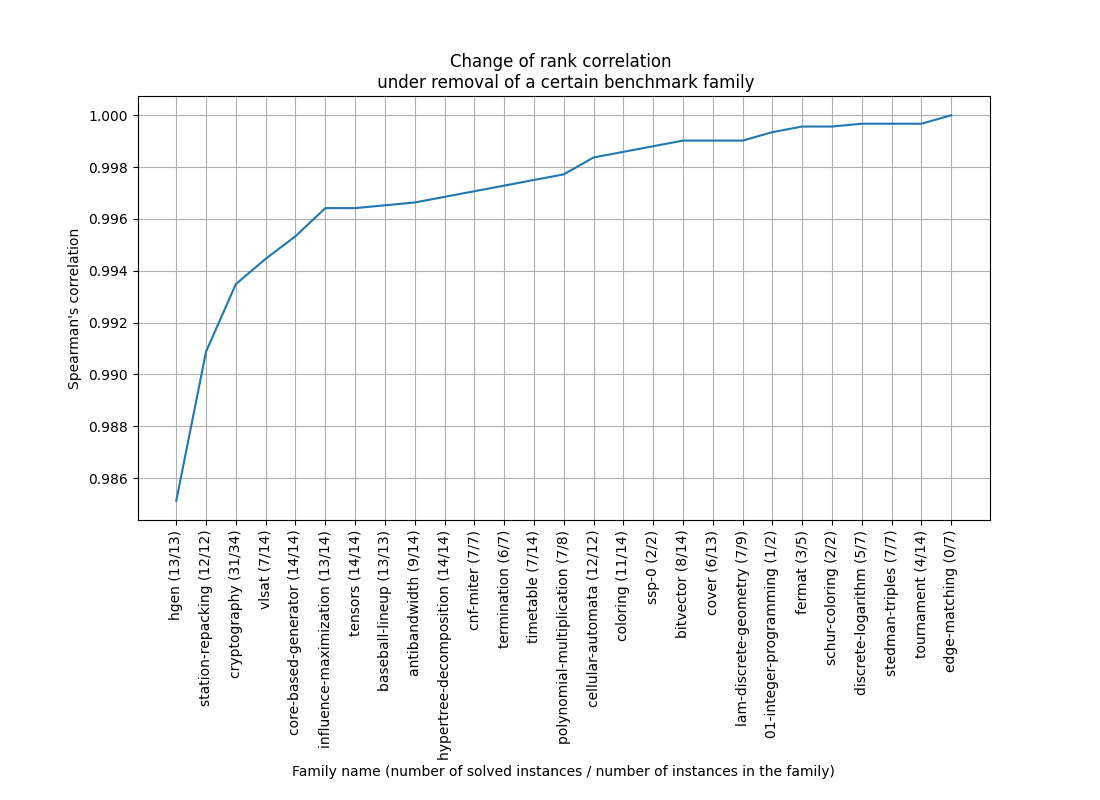
\includegraphics[width=0.9\textwidth]{stability/fam_leave_one_out_corr.png}
  \caption{Change of rank correlation under removal of individual benchmark families}
\end{figure}

Figure~\ref{fig:sampleFamily} shows the rank
correlation coefficient resulting from removing a complete benchmark family
instead of a random subset. As expected, removing a non random subset can have a
higher impact on the ranking even if it is small. Removing the $13$ benchmarks
from the \emph{hgen}-family results in a (still high) rank correlation of
$0.9895$. Additionally, the ranking of the top five solvers stays the same.
The individual removal of all other benchmarks families results in a rank correlation above $0.99$.

\section{Conclusion and Prospects}
\label{sec:conclusion}

All winning solvers of the \emph{Main} track periodically schedule runs of an SLS solver and import statistical information generated in unsuccessul SLS runs to reconfigure weights in their branching heuristics. 

As can be seen in the \emph{Parallel} track, it is hard to scale SAT solving beyond $32$ threads, as in some occassions the $32$ threaded version of the same solver outperformed its $64$ threaded counterpart. 
However, from the winner in the massively parallel \emph{Cloud} track, we can learn that classic all-to-all clause-sharing can be outperformed by a more sophisticated clause-sharing architecture. 

It is hard to integrate and test sophisticated state-of-the-art methods in an incremental SAT solver and thus solvers usually disable parts of their features in the incremental use-case. 
The winner of the \emph{Incremental Library} track showed that it is worth integrating full solver functionality in the incremental use-case. 

\subsection*{Future Competitions}

The \emph{Portfolio rule} has been established to prohibit participation of pure solver portfolios and to stimulate development of new code-bases. 
The rule was challenged in this competition, as it can be hurtful to cooperation in the community when solver authors use the work of other researchers as fully integrated sub-systems in their own code-base. 
Therefore, the \emph{Portfolio rule} will receive some refinement in future competitions. 

Many prominent applications of SAT use an \emph{incremental} SAT solver in their backend. 
Those incremental use-cases impose additional challenges on solver authors. 
The emergence of new fuzzing tools for incremental SAT solvers based on IPASIR can help researchers with also integrating and testing their methods in the incremental use-case.\footnote{\url{https://github.com/fkutzner/IncrementalMonkey}} 

The results of the \emph{Planning} track as well as our differentiated analysis of results highlight the individual contributions of many submissions. 
Our plan for future competitions is, to always run a special track for varying applications alongside the Main track. 


\section*{Acknowledgements}
The authors thank StarExec for their support and resources to run the Main and the Planning tracks, and Amazon Web Services 
for their support and resources to run the Parallel and Cloud tracks. 

Nils Froleyks is supported by the Austrian Science Fund (FWF) under projects
W1255-N23, S11408-N23 and by the LIT AI Lab funded by the State of Upper
Austria.
%
Marijn Heule is supported by the National Science Foundation (NSF) under grant CCF-2010951. 
%
Matti J\"arvisalo was financially supported by Academy of Finland grants 322869 and 328718.
%
Martin Suda was supported by the ERC Consolidator grant AI4REASON no. 649043 under the EU-H2020 programme,
the Czech Science Foundation project 20-06390Y, and the project RICAIP, no. 857306 under the EU-H2020 programme.



\bibliographystyle{elsarticle-num}
\bibliography{main}

\end{document}
